
\documentclass[12pt]{article}     
\usepackage{graphicx}
\graphicspath{{figures/}}
\usepackage[top=2.5cm, bottom=2.5cm, left=3cm, right=3cm]{geometry}
\usepackage{titlesec}
\usepackage{longtable}
\usepackage[table,xcdraw]{xcolor}
\usepackage{todonotes}
\usepackage{float}
\usepackage[T1]{fontenc}
\usepackage[utf8]{inputenc}
\usepackage{csquotes}
\usepackage{tocloft}
\usepackage{amssymb}
\renewcommand{\labelitemi}{\tiny$\blacksquare$} %For square itemized lists
\usepackage{caption} 
\captionsetup{labelsep=period}
\usepackage{verbatimbox} %To put program code in the center using Verbatim
\titlelabel{\thetitle.\quad}
\usepackage{times}
\usepackage{fancyhdr}
\setlength{\parindent}{0cm}
\usepackage{setspace}
\onehalfspacing
\setlength{\parskip}{\baselineskip}
\usepackage{amsmath} 
\usepackage{amsthm}
% Packages for building tables and tabulars 
\usepackage{array}
\usepackage{tabu}   % Wide lines in tables
\usepackage{xspace} % Non-eatable spaces in macros
\usepackage[colorlinks=true,linkcolor=blue]{hyperref}
\usepackage[all]{hypcap}
\usepackage{url}
% Packages for defining colourful text together with some colours
%\usepackage[table,xcdraw]{xcolor}
\definecolor{dkgreen}{rgb}{0,0.6,0}
\definecolor{gray}{rgb}{0.5,0.5,0.5}
\definecolor{mauve}{rgb}{0.58,0,0.82}
\definecolor{lightblue}{rgb}{0.95,0.97,1.0}
\definecolor{darkblue}{rgb}{0.90,0.92,1.0}
\usepackage{color}

% Standard package for drawing algorithms
% Since the thesis in article format we must define \chapter for
% the package algorithm2e (otherwise obscure errors occur) 
\let\chapter\section
\usepackage{algorithm2e}

% Macros that make sure that the math mode is set
\newcommand{\typeF}[1] {\ensuremath{\mathsf{type_{#1}}}\xspace}
\newcommand{\opDiv}{\ensuremath{\backslash \mathsf{div}}\xspace} 
\usepackage{listings}

\lstset{ 
  %language=python,                % the language of the code
  language=C++,
  basicstyle=\footnotesize,        % the size of the fonts that are used for the code
  %numbers=left,                   % where to put the line-numbers
  %numberstyle=\footnotesize,      % the size of the fonts that are used for the line-numbers
  numberstyle=\tiny\color{gray}, 
  stepnumber=1,                    % the step between two line-numbers. If it's 1, each line 
                                   % will be numbered
  numbersep=5pt,                   % how far the line-numbers are from the code
  backgroundcolor=\color{white},   % choose the background color. You must add \usepackage{color}
  showspaces=false,                % show spaces adding particular underscores
  showstringspaces=false,          % underline spaces within strings
  showtabs=false,                  % show tabs within strings adding particular underscores
  frame = lines,
  %frame=single,                   % adds a frame around the code
  rulecolor=\color{black},		   % if not set, the frame-color may be changed on line-breaks within 
                                   % not-black text (e.g. commens (green here))
  tabsize=2,                       % sets default tabsize to 2 spaces
  captionpos=b,                    % sets the caption-position to bottom
  breaklines=true,                 % sets automatic line breaking
  breakatwhitespace=false,         % sets if automatic breaks should only happen at whitespace
  %title=\lstname,                 % show the filename of files included with \lstinputlisting;
                                   % also try caption instead of title
                                   % also try caption instead of title
  keywordstyle=\color{blue},       % keyword style
  commentstyle=\color{dkgreen},    % comment style
  stringstyle=\color{mauve},       % string literal style
  escapeinside={\%*}{*)},          % if you want to add a comment within your code
  morekeywords={*,game, fun}       % if you want to add more keywords to the set
}

\usepackage{multirow}
\setlength{\tabcolsep}{0pt}
\newcolumntype{C}[1]{>{\centering\let\newline\\\arraybackslash\hspace{0pt}}m{#1-\arrayrulewidth\relax}}
\newcolumntype{L}[1]{>{\raggedright\let\newline\\\arraybackslash\hspace{0pt}}m{#1-\arrayrulewidth\relax}}

\usepackage{booktabs,fixltx2e}
\usepackage{tikz}
%used for ex. for m prime
\usepackage{flexisym}
\usepackage{footnote}

\usepackage{arydshln}
\usepackage{placeins}
\usepackage{enumitem}
\usepackage{cleveref}
\crefformat{footnote}{#2\footnotemark[#1]#3}
\usepackage{IEEEtrantools}

\begin{document}
\bstctlcite{IEEEexample:BSTcontrol}
%------------------------------TIITELLEHT---------------------------------
\thispagestyle{fancy}
\renewcommand{\headrulewidth}{0pt}
\renewcommand{\footrulewidth}{0pt}
\headheight = 57pt
\footskip = 11pt
\headsep = 0pt

\chead{
 \textsc{\begin{Large} %Tekst suurtähtedega ja suuremaks
	Tallinn University of Technology\\
	\end{Large} }
	Department of Computer Science\\	
	TUT Centre for Digital Forensics and Cyber Security
}
\vspace*{7 cm}

\begin{center}
ITC70LT\\[0cm]

Christian Ponti 144704\\
\vspace{15pt}
\begin{LARGE}
\textsc{What approach can be used to gain network access from outside by using ICMPv6?\\}
\end{LARGE}
\vspace{10pt}
Master Thesis\\[2cm]
\end{center}

\begin{flushright}
Supervisor: Bernhards Blumbergs\\[0cm]
MsC\\[0cm]
\end{flushright}

\cfoot{Tallinn 2016} 
\pagebreak

%---------------------------AUTORIDEKLARATSIOON-------------------------
\section*{\begin{center}
 Autorideklaratsioon
\end{center}}


Autorideklaratsioon on iga lõputöö kohustuslik osa, mis järgneb tiitellehele.
Autorideklaratsioon esitatakse järgmise tekstina:

Olen koostanud antud töö iseseisvalt. Kõik töö koostamisel kasutatud teiste autorite tööd, olulised seisukohad, kirjandusallikatest ja mujalt pärinevad andmed on viidatud. Käsolevat tööd ei ole varem esitatud kaitsmisele kusagil mujal.

Autor: [Ees$-$ ja perenimi]

[\today]
\pagebreak

%---------------------------ANNOTATION---------------------------------
\section*{\begin{center}
Annotatsioon
\end{center}}

Annotatsioon on lõputöö kohustuslik osa, mis annab lugejale ülevaate töö eesmärkidest, olulisematest käsitletud probleemidest ning tähtsamatest tulemustest ja järeldustest. Annotatsioon on töö lühitutvustus, mis ei selgita ega põhjenda midagi, küll aga kajastab piisavalt töö sisu. Inglisekeelset annotatsiooni nimetatakse Abstract, venekeelset aga


Sõltuvalt töö põhikeelest, esitatakse töös järgmised annotatsioonid:
\begin{itemize}
\item kui töö põhikeel on eesti keel, siis esitatakse annotatsioon eesti keeles mahuga $\frac{1}{2	}$ A4 lehekülge ja annotatsioon \textit{Abstract} inglise keeles mahuga vähemalt 1 A4 lehekülg;
\item kui töö põhikeel on inglise keel, siis esitatakse annotatsioon (Abstract)  inglise keeles mahuga $\frac{1}{2}$ A4 lehekülge ja annotatsioon eesti keeles mahuga vähemalt 1 A4 lehekülg;
\end{itemize}

Annotatsiooni viimane lõik on kohustuslik ja omab järgmist sõnastust:

Lõputöö on kirjutatud [mis keeles] keeles ning sisaldab teksti [lehekülgede arv] leheküljel, [peatükkide arv] peatükki, [jooniste arv] joonist, [tabelite arv] tabelit.
\pagebreak


%-----------------------------ABSTRACT-----------------------------------

\section*{\begin{center}
Abstract
\end{center}}
Võõrkeelse annotatsiooni koostamise ja vormistamise tingimused on esitatud eestikeelse annotatsiooni juures.

The thesis is in [language] and contains [pages] pages of text, [chapters] chapters, [figures] figures, [tables] tables.
\pagebreak

%---------------------Glossary of terms and Abbreviations---------------------

\section*{\begin{center}
Glossary of Terms and Abbreviations
\end{center}}

% \begin{tabular}{p{3 cm}ll}
% IPv6&Internet Protocol version 6\\
% ICMPv6&Internet Control Message Protocol version 6\\
% Node&ll\\
% NAT&dd\\
% IANA&Internet Assigned Numbers Authority\\
% BYID&Bring Your Own Device\\
% OS&Operating System\\
% IoT&Internet of Things\\
% rootkit&ff
% \end{tabular}

\begin{tabular}{L{3.3cm}L{12cm}}
\hdashline
\textit{Node}:&a device that implements IPv6\cite{rfc4861}.\\
\hdashline
\textit{Link}:&a communication facility or medium over which nodes can communicate at the link layer, i.e., the layer immediately below IPv6\cite{rfc4861}.\\
\hdashline
\textit{Interface}:&a node's attachment to a link\cite{rfc4861}.\\
\hdashline
\textit{Neighbors}:&nodes attached to the same link\cite{rfc4861}.\\
\hdashline
\textit{Prefix}:&a bit string that consists of some number of initial bits of an address\cite{rfc4861}.\\
\hdashline
\textit{On-link}:&an address that is assigned to an interface on a specified link\cite{rfc4861}.\\
\hdashline
\textit{Off-link}:&an address that is not assigned to any interfaces on the specified link\cite{rfc4861}.\\
\hdashline
\textit{Longest prefix match}:&the process of determining which prefix in a set of prefixes covers a target address. A target address is covered by a prefix if all of the bits in the prefix match the left-most bits of the target address. When multiple prefixes cover an address, the longest prefix is the one that matches\cite{rfc4861}.\\
\hdashline
\textit{Reachability}:&whether or not the one-way "forward" path to a neighbor is functioning properly. In particular, whether packets sent to a neighbor are reaching the IP layer on the neighboring machine and are being processed properly by the receiving IP layer\cite{rfc4861}.\\
\hdashline
\textit{Packet}:&an IPv6 header plus payload\cite{rfc4861}.\\
\hdashline
\textit{Link MTU}:&the maximum transmission unit, i.e., maximum packet size in octets, that can be conveyed over a link\cite{rfc4861}.\\
\hdashline
\textit{Path MTU}:&the minimum link MTU of all the links in a path between a source node and a destination node\cite{rfc4861}.\\
\hdashline
\textit{Multicast capable}:&a link that supports a native mechanism at the link layer for sending packets to all (i.e., broadcast) or a subset of all neighbors\cite{rfc4861}.\\
\hdashline
\textit{Point-to-point}:&a link that connects exactly two interfaces\cite{rfc4861}.\\
\hdashline
\end{tabular}

\begin{savenotes}
\begin{tabular}{L{3.3cm}L{12cm}}
\hdashline
\textit{Link-local address}:&a unicast address having link-only scope that can be used to reach neighbors\cite{rfc4861}.\\
\hdashline
\textit{All-nodes multicast address}:&the link-local scope address to reach all nodes, FF02::1\cite{rfc4861}.\\
\hdashline
\textit{All-routers multicast address}:&the link-local scope address to reach all routers, FF02::2\cite{rfc4861}.\\
\hdashline
\textit{Solicited-node multicast address}:&a link-local scope multicast address that is computed as a function of the solicited target's address. The function is chosen so that IP addresses that differ only in the most significant bits will map to the same solicited-node address thereby reducing the number of multicast addresses a node must join at the link layer\cite{rfc4861}.\\
\hdashline
\textit{Unspecified address}:&a reserved address value that indicates the lack of an address. It is never used as a destination address, but may be used as a source address if the sender does not know its own address. The 
unspecified address has a value of 0:0:0:0:0:0:0:0\cite{rfc4861}.\\
\hdashline
\textit{Covert Channel}:&is a communication paths that allow information transfer in violation of a system’s security policies. In the context of network protocols, covert channel communication is generally achieved by manipulating an overt communication\cite{lewandowski} \footnote{open to view or knowledge; not concealed or secret, \url{http://www.dictionary.com/browse/overt}, accessed 1.4.2016}.\\
\hdashline
\textit{Cover traffic}:&is the traffic that is being manipulated by covert channel participants\cite{lewandowski}.\\
\hdashline
\textit{Storage Covert Channel}:&manipulates a storage location in such a way that it conveys information to an observer. This definition was initially applied only to covert channels within a single machine or at least with a shared storage location. It was then extended to network covert channels and in this context, a storage channel is understood to be a channel that relies on modification of network traffic content\cite{lewandowski}.\\
\hdashline
\textit{Active Warden}:&is positioned so that it can observe and modify network traffic in its area of responsibility. The task of active wardens is to prevent and disrupt covert channel communication by modifying the content of network traffic\cite{lewandowski}\\
\hdashline
\end{tabular}
\end{savenotes}

\begin{savenotes}
\begin{tabular}{L{3.3cm}L{12cm}}
\hdashline
\textit{Policy}:&a formal, brief, and high-level statement or plan that embraces an organization's general beliefs, goals, objectives, and acceptable procedures for a specified subject area \footnote{\label{policy}\url{http://www.slu.edu/its/policies-and-processes}, accessed 1.4.2016}.\\
\hdashline
\textit{Standard}:&a mandatory action or rule designed to support and conform to a policy \cref{policy}.\\
\hdashline
\textit{Procedure}:&procedures describe the process: who does what, when they do it, and under what criteria \cref{policy}.\\
\hdashline
\textit{System Preservation}:&guarantees that the stegomessage is well formed within the rules of the protocol; the actual meaning of the stegomessage may be different than the original cover\cite{lucena2}.\\
\hdashline
\textit{Semantic Preservation}:&means that, as observed at a point along the message’s path through the network, the stegomessage has the same meaning as the original cover\cite{lucena2}.\\
\hdashline
\end{tabular}
\end{savenotes}



\pagebreak

\tableofcontents
\newpage
\listoffigures
\pagebreak
\listoftables
\pagebreak

\section{Introduction}
\label{sec:1}


IPv6 is the designated successor of IPv4, a protocol specified and implemented in a context with a limited number of users and hosts, most of them circumscribed to the scientific world. The need of a new protocol arose because of a changed context: the evolution of new powerful devices and their spread in many field of the society, which in turn modified the behavior and the requests of new entities, being them individuals or big organizations. The new IP protocol has been specified and redesigned in many aspects, taking in consideration the evolution of the requirements and the future needs of the involved actors.

IPv6\cite{rfc2460}, with respect to his predecessor, changed in many aspects. The headers have been modified to accommodate new functionality and improved capabilities, mainly it provides ``expanded addressing capabilities'', ``header format simplification'', ``improved support for extensions and options'', ``flow labeling capability'', and ``authentication and privacy capabilities''. One of the most relevant aspect is the increased address space from 32 bits to 128 bits, which deals with the demand of new communicating devices to fulfill organization's requirements.

Despite IPv6 specifications have been formalized in 1998, its spread and adoption by the world community is far from being accomplished. Among the many possible reasons that could explain this behavior, two of them deserve particular attention. The first one is related to the depletion of address space, which has been mitigated by the introduction of Network Address Translation (NAT)\cite{rfc3022}: the use of NAT allows to use a private, not routeable, address space for the internal network of an organization, and the use of one, or limited number, public IPv4 address at the network boundary. This technique mitigated the need to request an IPv6 128 bits address by organizations, because their requirements to allocate new IPv4 address from IANA\footnote{\url{http://www.iana.org/}} have been reduced. The second reason is related to the applications and services offered by organizations. These applications have been written for, and tested against, IPv4. Many of them represents IT assets which are critical for the business assets and goals of enterprises: the introduction of new applications written for IPv6 represents a great effort in terms of financial investment, time for implementation and testing, and use of enterprises' resources.

The IPv6 world is composed by a number of protocols, which are used by nodes to fulfill their requirements: for some of them it is possible to find similar functionality in IPv4, while others are completely new protocols. In this set of protocols, one of them deserves particular attention: ICMPv6.

ICMPv6, despite it shares almost the same naming convention with respect with the predecessor, it is a new protocol, which make it a critical subject of research by the scientific community. The reasons behind its criticality arise because it holds some functions which are similar in ICMP (e.g. Echo Request), but at the same time it introduces a number of new functionalities, and responsibilities, for the correct behavior of an IPv6 node.

ICMP has been used by IPv4 to manage error and informational messages to allow for a better management and troubleshooting of the network.  This protocol has been tested for many years, with the identification of vulnerabilities which can be potentially be exploited by malicious actors. Many best practices \footnote{\url{http://www.cisco.com/c/en/us/support/docs/ip/access-lists/13608-21.html\#anc29}, accessed 20.03.2016} \footnote{\url{http://www.cisco.com/c/en/us/about/security-center/firewall-best-practices.html\#\_Toc332805964}, accessed 20.03.2016} suggested to filter ICMPv4 messages at network boundaries to mitigate the risk of the exploitation of some vulnerabilities without compromising the network functionalities. Nowadays the network evolved in more sophisticated designs, and new concepts, like Bring Your Own Device (BYOD) and wireless networks, partially obsolete the very same concept of boundaries, bringing new threats to the internal network. The security controls could no more be applied only at the boundaries, but must be introduced in other segments of the network. This new security controls applies to the ICMPv4 protocol as well, and filtering must be introduced where such messages are not strictly required by network administrators.

``ICMPv6 is used by IPv6 nodes to report errors encountered in processing packets, and to perform other internet-layer functions, such as diagnostics (ICMPv6 Echo). ICMPv6 is an integral part of IPv6, and the base protocol (all the messages and behavior required by this specification) MUST be fully implemented by every IPv6 node''\cite{rfc4443}.

This paragraph of RFC 4443 describes broadly the purpose of ICMPv6, but the most important part is the last sentence, which states that the base protocol must be fully implemented by every IPv6 node. In the RFC terminology, the word “MUST, or the terms REQUIRED or SHALL, mean that the definition is an absolute requirement of the specification“\cite{rfc2119}. The real distinction between ICMPv4 and ICMPv6 in this context is formal: RFC 792 states that ``ICMP [...] must be implemented by every IP module''\cite{rfc792}, which means that an implementation is required. The ICMPv6 specification is more precise because it refers to every IPv6 node, which covers the implementation inside the module, but also, with the concept of node, implies that the node must be able to use its functions.

This is a fundamental distinction, because the best practices in use with ICMPv4, with ICMPv6 are no more relevant, at least with some message types. As it is written in this paper\cite{chak}, which cites RFC 4861\cite{rfc4861}, ``ICMPv6 is used for basic functionalities and used by other IPv6 protocols [...] Neighbor Discovery Protocol is a protocol used with IPv6 to perform various tasks like router discovery, stateless automatic address configuration of a node, neighbor discovery, duplicate address detection, determining the Link Layer addresses of other nodes, address prefix discovery, and maintaining routing information about the paths to other active neighbor nodes''.

This is the first critical point to consider: despite version 4 and version 6 of the ICMP protocol have some similar functions, they are different protocols. ICMPv6 is not a protocol modified to adapt itself to IPv6, a new analysis must be performed in an exhaustive way taking into account new scenarios, and new best practices must be applied to mitigate the risk of exploitation of new vulnerabilities related to its functionalities.

Another important aspect to take into consideration when dealing with IPv6 in general, and with ICMPv6, is the transition from version 4 to version 6. For the aforementioned reasons, many organizations delayed as much as they could the deployment of an IPv6 native Internet connectivity. Nevertheless the scientific community continued to improve the new version and its related protocols, and Operating Systems (OS) started to include them in their network implementations. At the same time, techniques to allow a slow transition have been developed: examples of that are the dual stack, the presence and coexistence of both protocol versions in the same node, or the encapsulation of IPv6 inside IPv4, in those network segments where IPv6 has not been deployed yet. Additionally, in many OS, IPv6 is active by default and preferred over IPv4.

These aspects must not be underestimated and show again how critical and urgent is an in-depth analysis of ICMPv6: not only this protocol is fundamental for IPv6 and the best practices can be used only against the previous version, but it is already present and activated in OS that users employ in their everyday life. This last distinction is very important because it introduces another aspect to take into account: network administrator and security officer must not deal only with threats deriving from the exploitation of technical vulnerabilities, but also with behavioral procedures shaped around years of practice. IPv6 and ICMPv6 are not protocols that will be introduced in the future, they are already present in this transition period and we must deal with them now. Countermeasures must be in place, at the network boundaries and inside critical network segments above all, that take into consideration version 6 of the protocols. Such countermeasures must follow new best practices carefully shaped around the new version.

The underlined elements, the differences between the two ICMP version and the transition period with the coexistence of IPv4 and IPv6, lead to another topic: the impact of the full deployment of IPv6, and ICMPv6, and the implications for the involved actors, being them users, enterprises, states, or malicious actors.

The scientific community has been involved in the specification, in the improvement, and testing of the protocols since time. But, with respect with the preceding version of the protocols, version 6 of the suite must deal with a very different situation. The electronic communication is spread around the world in a pervasive way, and the near future, with the Internet of Things (IoT) \footnote{IoT, \url{http://www.theinternetofthings.eu/what-is-the-internet-of-things}, accessed 21.03.2016}, will further the spread. ICMPv6, and IPv6, will be fully deployed in a world strongly dependent on the electronic communication, where critical infrastructures (CI) must be managed and protected, where enterprises relies on its IT infrastructure to support their business assets, and where users are tight to their online experience for their everyday needs. This change in the very basic infrastructure of the network will have an impact which has no terms of comparison with respect to IPv4, where the initial small amount of users allowed to discover the concept of security and to learn by experience. The transition period, which introduced some security issues, in this case works as a mitigation technique to allow researcher to test the protocols in an exhaustive way, without waiting that the fully deployed IPv6 infrastructures reveals potential weaknesses.

This urgency can be better understood by taking into consideration the evolution of the threats, the sophistication of malware, and the malicious actors involved in the research of vulnerabilities to exploit, as well as their purposes and means to reach their goals.

The term Advanced Persistent Threat (APT) is used to define ''any sophisticated adversary engaged in information warfare in support of long-term strategic goals``\cite{apt}. One of the main characteristic of APT detected in the wild is the sophistication of the attack. One example is the Uroburos rootkit\cite{uroburos}, which ''modular structure allows extending it with new features easily, which makes it not only highly sophisticated but also highly flexible and dangerous``. The analysis of the rootkit suggests that ''the development of a framework like Uroburos is a huge investment`` and ''that it was designed to target government institutions, research institutions or companies dealing with sensitive information as well as similar high-profile targets``. There are other example of APT that suggested an evolution of the threat landscape, like Stuxnet\cite{stuxnet}. Even if the aforementioned malware do not target directly IPv6, they share a common characteristic which is important to underline: the sophistication, the investment behind them, and the presence of an Advanced Persistent Adversary (APA)\cite{apa}, term that ''depicts not only the threat, but the threat actors as well``.

The evolution of the threat landscape depicts a situation where APA, often associated with groups sponsored by state actors, have a remarkable budget to develop very sophisticated attacks to reach their goals. In the current situation, given the impact that the full deployment of IPv6 will have, those actors have the resources and the motivation to research and discover vulnerabilities in IPv6, ICMPv6, and other protocols involved. 
Moreover, if this research will succeed, APA can gain a considerable advantage over their opponents, because a possible vulnerability at network layer may allow to bypass more easily the security mechanisms in place and give more robust mechanisms to stay undetected for longer.

While research and tests on ICMPv6 are an ongoing process, the urgency and criticality of the subject require a more in-depth analysis which take into account the full deployment, but also the transition period. To pursue this goal it is important to start from the specifications of the protocol, the RFCs. Those documents represent a guideline, the result of an agreement between many stakeholders. As a guideline, there is no guarantee that the implementation will follow the suggestion, even in the sections specified with a ''must``.

It is worth to underline the contribution of this research. The first contribution is to produce the necessary awareness with regard to IPv6 and ICMPv6. This is the starting point to understand the need to analyze the protocols in detail. Furthermore, it is important to see the big picture, which include not only ICMPv6, but also its relationship with the devices involved in the communication, the target hosts, and the firewalls through which the packets must transit. Firewalls are devices configured by human beings, which may commit mistakes and use different best practices. Each configuration can produce a different scenario, which is worth to analyze because in the real world each system may differ from another, and the goal of an APA is to find these slight differences between them to take advantage. This work's contribution is an analysis of different scenarios where the use of the ICMPv6 protocol could arise different security issues, with respect to the configuration of network boundary devices. A scenario-based experiment needs also a test set, based on RFC specifications, and the implementation of a software to conduct the experiments, which also represent a contribution of this research.

The novelty of this research resides in the scenario-based experiment, which involves the identification of a test set based on the RFCs specifications, to find possible vulnerabilities that can be exploited. Furthermore, the tests must consider both directions of the network flow, from the outside to the internal network, and from the internal and trusted network to the outside. The traffic traveling in both directions must cross a network boundary device, which is a necessary condition to consider a potential vulnerability as such. The reason behind the novelty of this approach is that, as this research will underline in next chapter, other researches consider only one traffic flow direction, or the compliance with the protocol itself of most implementation, without considering network boundary devices, which, taking into account the transition period, may or may not be configured to cope with IPv6 and the related protocols. Furthermore, this research is developed from a penetration testing point of view. Penetration testing is a process with the aim to gain access to resources with the permission of the owner\cite{penTesting}. This point of view is important, because the process simulates what an attacker may do while attempting to gain access to a company's resources. As the research will point out, a vulnerability may exist, but its exploitation may depend on the configuration of a firewall, which might reduce the probability of the exploitation by a malicious actor.

The next chapters of this work will explore the background, the specification inside RFCs, and the related work(see~\ref{sec:2}), which includes existing tools and projects to test ICMPv6, and a review of the literature. Then the analysis proceeds with definition of the methodology(see~\ref{sec:3}) of this research, which is based on the scientific method of the experimentation; the chapter includes the motivation behind this choice and behind the choice of the technology to conduct the experiments. The implementation is the next chapter(see~\ref{sec:4}), which deal with the details of the technology, followed by the experiment(see~\ref{sec:5}), which describes the set of performed tests. The chapter related to the results(see~\ref{sec:6}) includes a discussion about the results of the experiment and its meaning. Finally, the conclusions(see~\ref{sec:7}) summarizes the research, discuss about suggestions and future work.

 

\pagebreak
%------------------------------BACKGROUND AND RELATED WORK-----------------------------------
\section{Background and Related Work}
\label{sec:2}


\subsection{Background}
\label{sub:background}

``The Internet Standards process is an activity of the Internet Society\footnote{\url{http://www.internetsociety.org/}} that is organized and managed on behalf of the Internet community by the Internet Architecture Board (IAB)\footnote{\url{https://www.iab.org/}} and the Internet Engineering Steering Group (IESG)\footnote{\url{https://www.ietf.org/iesg/}}. [...] an Internet Standard is a specification that is stable and well-understood, is technically competent, has multiple, independent, and interoperable implementations with substantial operational experience, enjoys significant public support, and is recognizably useful in some or all parts of the Internet. [...] Each distinct version of an Internet standards-related specification is published as part of the Request for Comments (RFC) document series.  This archival series is the official publication channel for Internet standards documents and other publications of the IESG, IAB, and Internet community.''\cite{rfc2026}

This work starts by analyzing the RFCs related to ICMPv6, which specify the protocol and the features to which each implementation must adhere. The main goal of an agreement on a protocol is interoperability \footnote{\url{http://www.merriam-webster.com/dictionary/interoperability}}, but, since this is not a binding process, and even though implementations follow the main specifications, it is always possible that some of them do not adhere completely. This could lead to some interoperability issues, which may introduce vulnerabilities in the protocol.

The background of this research is represented by two RFCs, ``Internet Control Message Protocol (ICMPv6) for the Internet Protocol Version 6 (IPv6) Specification''\cite{rfc4443}, and ``Neighbor Discovery for IP version 6 (IPv6)''\cite{rfc4861}. These two RFCs specify the general header for ICMPv6 messages, and each specific message header to which each implementation must adhere.

The IPv6 specification\cite{rfc2460} is only partially in the scope of this research, but it must be mentioned, because of its tight relationship with ICMPv6, and because in each ICMPv6 message type specification some of its fields are cited, as it will be underlined later in the chapter.

RFCs use a specific set of words to express the requirements of the implementations \cite{rfc2119}. Words like ``must'', or ``should'' have a particular meaning, as expressed in the cited document, that should be well understood by implementors. The reason is that a lack of compliance may lead to the introduction of some vulnerabilities, where a node is expecting a particular behavior from another peer, while the peer's implementation follows slightly different specifications. This research, inside next sections, will try to underline where, under each message type, and along the general specifications (e.g. general processing rules), it is possible to insert vulnerabilities in the protocol if the interpretation of the specifications were different between the implementations.

Since the list of possibilities may be long, this research will use criteria in order to generate a subset of specification to test. The followed mechanism is to first select specifications and insert them into a set of tables, each related to a specific message, and then select from each table the test to be performed during the experiment. The criteria are presented at the end of this chapter, after the related works' analysis.

\pagebreak

\subsubsection{RFC 2460}
\label{subsub:2460}
The table (see~\ref{table:IPv6}) shows the specification of the IPv6 header. From the point of view of this research, there are four interesting fields which are strictly involved in the ICMPv6 specification:
\vspace{-15pt}
\begin{itemize}[noitemsep,topsep=0pt,partopsep=0pt]
 \item \textbf{Next Header}:\quad 8-bit, identifies the type of header immediately following the IPv6 header. Uses the same values as the IPv4 Protocol field. The ICMPv6 value is 58. The complete list is available on IANA's website\footnote{\url{http://www.iana.org/assignments/protocol-numbers/protocol-numbers.xhtml}, accessed on 27.03.2016}
 \item \textbf{Hop Limit}:\quad 8-bit, decremented by 1 by each node that forwards the packet. The packet is discarded if Hop Limit is decremented to zero.
 \item \textbf{Source Address}:\quad 128-bit address of the originator of the packet.
 \item \textbf{Destination Address}:\quad 128-bit address of the intended recipient of the packet.
\end{itemize}


\subsubsection{RFC 4443}
\label{subsub:4443}

The Internet Control Message Protocol (ICMPv6) for the Internet Protocol Version 6 (IPv6) Specification categorizes two broad type of messages, error and informational messages.

As shown in the table (see~\ref{table:ICMPv6}), the general ICMPv6 header format is composed by an 8 bit \textbf{type} field, an 8 bit \textbf{code} field, and a 16 bit \textbf{checksum} field. The message body suggests specific header fields which are characteristic of each message type.

ICMPv6 messages are categorized by its type field, while the code field in this specification identifies a specific message under the category.

Error messages are characterized by a 0 in the high order bits of the type field, which gives a value range between 0 and 127. Informational message are instead characterized by a 1 in the high order bits, for a possible 
value range between 128 and 255.

\begin{savenotes}
\begin{table}[h]
\centering
\begin{tabular}{|C{1.5cm}C{1.5cm}C{1.5cm}C{1.5cm}C{1.5cm}C{1.5cm}C{1.5cm}C{1.5cm}|}
\hline
\multicolumn{2}{|C{3.0cm}}{\cellcolor{darkblue} Type}&\multicolumn{2}{|C{3.0cm}|}{\cellcolor{lightblue} Code}&\multicolumn{4}{C{6.0cm}|}{\cellcolor{darkblue} Checksum}\\
\hline
\rowcolor{lightblue}
\multicolumn{8}{|c|}{}\\
\rowcolor{lightblue}
\multicolumn{8}{:c:}{\multirow{-2}{*}{\hfil Message Body}}\\
\hdashline
%\hline
\end{tabular}
\caption{ICMPv6 General Header Format}
\label{table:ICMPv6}
\end{table}
\end{savenotes}

The next two table (see~\ref{table:ICMPv6ErrorMessages} and~\ref{table:ICMPv6InformationalMessages}) summarize the type of ICMPv6 messages described in this RFC.

\begin{savenotes}
\begin{table}[!htpb]
\centering
\addtolength{\tabcolsep}{3pt}
\begin{tabular}{|L{3.0cm}|L{8.0cm}|}
\rowcolor{lightblue}
\hline
Type field&Error Message\\
\hline
1&Destination Unreachable\\
\hline
2&Packet Too Big\\
\hline
3&Time Exceeded \\
\hline
4&Parameter Problem\\
\hline
100&Private experimentation\\
\hline
101&Private experimentation\\
\hline
127&Reserved for expansion of ICMPv6 error messages\\
\hline
\end{tabular}
\caption{ICMPv6 Error Messages}
\label{table:ICMPv6ErrorMessages}
\end{table}
\end{savenotes}

\begin{savenotes}
\begin{table}[!htpb]
\centering
\addtolength{\tabcolsep}{3pt}
\begin{tabular}{|L{3.0cm}|L{8.0cm}|}
\rowcolor{lightblue}
\hline
Type field&Informational Message\\
\hline
128&Echo Request\\
\hline
129&Echo Reply\\
\hline
200&Private experimentation\\
\hline
201&Private experimentation\\
\hline
255&Reserved for expansion of ICMPv6 informational messages\\
\hline
\end{tabular}
\caption{ICMPv6 Informational Messages}
\label{table:ICMPv6InformationalMessages}
\end{table}
\end{savenotes}
The RFC, besides ICMPv6 fields, gives directives also for IPv6 fields of interest. For all the error messages and Echo Reply is the Destination Address field, which is ``copied from the Source Address field of the invoking packet''. For an Echo Request, the IPv6 field is ``any legal IPv6 address''.

Besides type and code fields, another field is common to all the ICMPv6 messages: the checksum. The checksum is ``used to detect data corruption in the ICMPv6 message and parts of the IPv6 header'' and ``is the 16-bit one's complement of the one's complement sum of the entire ICMPv6 message, starting with the ICMPv6 message type field, and prepended with a pseudo-header of IPv6 header fields''. The procedure implies to sum up the binary values of 16 bit at a time, and invert the bit values of the final result.

The RFC includes a ``Message Processing Rules'' section, which underlines the rules that a node must observe while processing an ICMPv6 message. The complete list is in table ~\ref{table:4443ProcRules} in Appendix 2.

During the preparation for the experiment it is important to identify tests that may lead to unexpected, from the RFC specification point of view, results. One example of that, taking the first rule in the aforementioned table, may be:\newline
what would happened in the case that an ICMPv6 error message of unknown type is received at its destination, and it is passed to the upper-layer process with a forged malicious payload?

As this research will show, some test may be spread across different scenarios, while other are more suitable to be performed only in a specific scenario; the example above is a good candidate for an outside-to-inside direction scenario, in order to test the behavior of an internal node.


\textbf{Destination Unreachable}

The first inspected message type is Destination Unreachable. Its purpose is to generate an error ``in response to a packet that cannot be delivered to its destination address for reasons other than congestion''.

For a detailed view of the header, table (see~\ref{table:destUnreach}) in \ref{Appendix 1}.

The table (see~\ref{table:destUnreachCodes}) summarizes the type and code fields of the header, with the corresponding code name of the message.

\begin{savenotes}
\begin{table}[!ht]
\centering
\addtolength{\tabcolsep}{3pt}
\begin{tabular}{|C{1cm}|C{1cm}|L{12.0cm}|}
\rowcolor{lightblue}
\hline
Type&Code&Description\\
\hline
\multirow{7}{*}{1}&0&No Route to Destination\\ \cline{2-3}
&1&Communication with destination administratively prohibited\\ \cline{2-3}
&2&Beyond scope of source address\\ \cline{2-3}
&3&Address unreachable\\ \cline{2-3}
&4&Port unreachable\\ \cline{2-3}
&5&Source address failed ingress/egress policy\\ \cline{2-3}
&6&Reject route to destination\\ \cline{2-3}
\hline
\end{tabular}
\caption{Destination Unreachable Codes}
\label{table:destUnreachCodes}
\end{table}
\end{savenotes}

The Unused field accordingly to the RFC must be initialized to zero by the originator and ignored by the receiver.

The following illustrates the meaning behind codes and description:
\vspace{-15pt}
\begin{enumerate}[noitemsep,topsep=0pt,partopsep=0pt]
 \item \textbf{No Route to Destination}: lack of a matching entry in the forwarding node's routing table
 \item \textbf{Communication with destination administratively prohibited}: administrative prohibition (e.g., a ``firewall filter'')
 \item \textbf{Beyond scope of source address}: the destination is beyond the scope of the source address (e.g., when a packet has a link-local source address and a global-scope destination address)
 \item \textbf{Address unreachable}: the reason for the failure to deliver cannot be mapped to any of other codes
 \item \textbf{Port unreachable}: generated in response to a packet for which the transport protocol (e.g., UDP) has no listener
 \item \textbf{Source address failed ingress/egress policy}: the packet with this source address is not allowed due to ingress or egress filtering policies
 \item \textbf{Reject route to destination}: the route to the destination is a reject route (may occur if the router has been configured to reject all the traffic for a specific prefix)
\end{enumerate}

\textbf{Packet Too Big}

A Packet Too Big must be sent by a router in response to a packet that it cannot forward because the packet is larger than the MTU of the outgoing link.

The table (see~\ref{table:packettoobig}) in Appendix 1 shows the header fields.

For this message the type field must always be 2 and the code set to 0 and ignored by the receiver. The MTU value represent ``the Maximum Transmission Unit of the next-hop link''.

\textbf{Time Exceeded Message}

The table (see~\ref{table:timeExceeded}) in Appendix 1 underlines the header fields of this type of message, table \ref{table:timeExceededCodes} shows the codes.

\begin{savenotes}
\begin{table}[!htpb]
\centering
\addtolength{\tabcolsep}{3pt}
\begin{tabular}{|C{2.0cm}|C{2.0cm}|L{6.5cm}|}
\rowcolor{lightblue}
\hline
Type&Code&Description\\
\hline
\multirow{2}{*}{3}&0&Hop limit exceeded in transit\\ \cline{2-3}
&1&Fragment reassembly time exceeded \\ \cline{2-3}
\hline
\end{tabular}
\caption{Time Exceeded Codes}
\label{table:timeExceededCodes}
\end{table}
\end{savenotes}

If a router receives a packet with a Hop Limit of zero, or if a router decrements a packet's Hop Limit to zero, it must discard the packet and originate an ICMPv6 Time Exceeded message with Code 0 to the source of the packet. An ICMPv6 Time Exceeded message with Code 1 is used to report fragment reassembly timeout.

\textbf{Parameter Problem Message}

``If an IPv6 node processing a packet finds a problem with a field in the IPv6 header or extension headers such that it cannot complete processing the packet, it must discard the packet and should originate an ICMPv6 Parameter Problem message to the packet's source, indicating the type and location of the problem''.

The table (see~\ref{table:paramProb}) in Appendix 1 underlines the header fields of this type of message.

Table \ref{table:paramProbCodes} shows a mapping between each code and a description of the error.

\begin{savenotes}
\begin{table}[!htpb]
\centering
\addtolength{\tabcolsep}{3pt}
\begin{tabular}{|C{1.0cm}|C{1.0cm}|L{8.0cm}|}
\rowcolor{lightblue}
\hline
Type&Code&Description\\
\hline
\multirow{3}{*}{4}&0&Erroneous header field encountered\\ \cline{2-3}
&1&Unrecognized Next Header type encountered\\ \cline{2-3}
&2&Unrecognized IPv6 option encountered \\
\hline
\end{tabular}
\caption{Parameter Problem Codes}
\label{table:paramProbCodes}
\end{table}
\end{savenotes}
Accordingly to the specification, the pointer field ``identifies the octet offset within the invoking packet where the error was detected. The pointer will point beyond the end of the ICMPv6 packet if the field in error is beyond what can fit in the maximum size of an ICMPv6 error message''.

\textbf{Echo Request}

The RFC states that each node must implements an Echo mechanism in order to produce Echo Requests and answer with Echo Replies. It also mentions the implementation of an application layer interface, for diagnostics purposes, to originate requests and receive replies.

The table (see~\ref{table:echoReq}) in Appendix 1 shows the header fields of an Echo Request message.

An Echo Request code is always 0. Identifier and Sequence Number are considered helping fields, which, in fact, could be expected to be zero, as depicted in table \ref{table:echoReqFields}.
\begin{savenotes}
\begin{table}[!htpb]
\centering
\addtolength{\tabcolsep}{3pt}
\begin{tabular}{|L{2.0cm}|L{10.0cm}|}
\rowcolor{lightblue}
\hline
Field&Value/Description\\
\hline
Type&128\\
\hline
Code&0\\
\hline
Identifier&An identifier to aid in matching Echo Replies to this Echo Request. May be zero.\\
\hline
Sequence Number&A sequence number to aid in matching Echo Replies to this Echo Request. May be zero.\\
\hline
Data&Zero or more octets of arbitrary data.\\
\hline
\end{tabular}
\caption{Echo Request Fields}
\label{table:echoReqFields}
\end{table}
\end{savenotes}

\textbf{Echo Reply}

For the Echo Reply Header (see~\ref{table:echoRep}), while table \ref{table:echoRepFields} shows the fields with the value, where present, or the function.

\begin{savenotes}
\begin{table}[!htpb]
\centering
\addtolength{\tabcolsep}{3pt}
\begin{tabular}{|L{2.0cm}|L{11.0cm}|}
\rowcolor{lightblue}
\hline
Field&Value/Description\\
\hline
Type&129\\
\hline
Code&0\\
\hline
Identifier&The identifier from the invoking Echo Request message.\\
\hline
Sequence Number&The sequence number from the invoking Echo Request message.\\
\hline
Data&The data from the invoking Echo Request message.\\
\hline
\end{tabular}
\caption{Echo Reply Fields}
\label{table:echoRepFields}
\end{table}
\end{savenotes}
The RFC reiterate the implementation of the same mechanism as underlined in the Echo Request. In addition, it highlights that if the message is in response to a request to the unicast address of the node, the source address of the Echo Reply must be copied from the destination address field of the Echo Request.

An Echo Reply should be also originated in the case that the Request has been made to an IPv6 multicast or anycast address, in this case with the source address of the interface that received the message.

The data, which has no limitations in size, must be the same which has been received inside the Echo Request.


\subsubsection{RFC 4861}
\label{subsub:4861}

The Neighbor Discovering Protocol has many functionalities and it is used by an IPv6 nodes in order to determine the link-layer address of neighbors, hosts and routers, and to discover which router is able to forward their packets to another off-link networks. In addition, it is used as a reachability mechanism to determine if a host is still alive.

The RFC defines five additional messages, characterized by the type field (for these messages the code is always zero), as summarized in table \ref{table:4861Messages}.

\begin{savenotes}
\begin{table}[!htpb]
\centering
\addtolength{\tabcolsep}{3pt}
\begin{tabular}{|C{3.0cm}|L{8.0cm}|}
\rowcolor{lightblue}
\hline
Type field&Message\\
\hline
133&Router Solicitation\\
\hline
134&Router Advertisement\\
\hline
135&Neighbor Solicitation\\
\hline
136&Neighbor Advertisement\\
\hline
137&Redirect\\
\hline
\end{tabular}
\caption{RFC 4861 Messages}
\label{table:4861Messages}
\end{table}
\end{savenotes}

This RFC defines in addition five options, with the possibility to be extended in the future, that ``provide a mechanism for encoding variable length fields, fields that may appear multiple times in the same packet, or information that may not appear in all packets''. Options defined in the document are:
\vspace{-15pt}
\begin{itemize}[noitemsep,topsep=0pt,partopsep=0pt]
 \item Source Link-Layer Address
 \item Target Link-Layer Address
 \item Prefix Information
 \item Redirected Header
 \item MTU
\end{itemize}


\textbf{Router Solicitation}

The function of a Router Solicitation message, for a host, is to inform a router to generate a Router Advertisement. The format of a Router Solicitation is shown in Appendix 1 (see~\ref{table:routerSolicit}).

Router Solicitation specifies three IPv6 fields:

\begin{tabular}{L{4.0cm}L{11.5cm}}
 \hdashline
 Source Address&An IP address assigned to the sending interface, or the unspecified address if no address is assigned to the sending interface.\\
 \hdashline
 Destination Address&Typically the all-routers multicast address.\\
 \hdashline
 Hop Limit&255\\
 \hdashline
\end{tabular}

\vspace{15pt}
The next table (see~\ref{table:routerSolfields}) summarizes the requirements of the fields.\\
\begin{savenotes}
\begin{table}[!htpb]
\centering
\addtolength{\tabcolsep}{3pt}
\begin{tabular}{|L{3.0cm}|L{10.0cm}|}
\rowcolor{lightblue}
\hline
Field&Value/Description\\
\hline
Type&133\\
\hline
Code&0\\
\hline
Reserved&This field is unused. It must be initialized to zero by the sender and must be ignored by the receiver.\\
\hline
\rowcolor{lightblue}
\multicolumn{2}{|c|}{Valid Options}\\
\hline
Source link-layer address &The link-layer address of the sender, if known.\\
\hline
\end{tabular}
\caption{Router Solicitation Fields and Options}
\label{table:routerSolfields}
\end{table}
\end{savenotes}


\textbf{Router Advertisement}

Router Advertisement are sent by routers periodically, or in response to a Router Solicitation, to help hosts in their configuration processes. Examples of such processes are the mechanism to configure their addresses, how to obtain information about DNS servers, prefix information for the link.

The table \ref{table:routerAdvert} in Appendix 1 shows the header of a Router Advertisement.

Router Advertisement specifies three IPv6 fields:

\begin{tabular}{L{4.0cm}L{11.5cm}}
\hdashline
 Source Address&must be the link-local address assigned to the interface from which this message is sent.\\
 \hdashline
 Destination Address&Typically the Source Address of an invoking Router Solicitation or the all-nodes multicast address.\\
 \hdashline
 Hop Limit&255\\
 \hdashline
\end{tabular}

\vspace{15pt}
The table (see~\ref{table:routerAdvfields}) summarizes the fields with their specifications.

\begin{savenotes}
\begin{table}[!htpb]
\centering
\addtolength{\tabcolsep}{3pt}
\begin{tabular}{|L{3.0cm}|L{11.6cm}|}
\rowcolor{lightblue}
\hline
Field&Value/Description\\
\hline
Type&134\\
\hline
Code&0\\
\hline
Cur Hop Limit&The default value that should be placed in the Hop Count field of the IP header for outgoing IP packets. A value of zero means unspecified\\
\hline
M&"Managed address configuration" flag. When set, it indicates that addresses are available via Dynamic Host Configuration Protocol\\
\hline
O&"Other configuration" flag. When set, it indicates that other configuration information is available via DHCPv6.\\
\hline
Reserved&It must be initialized to zero by the sender and must be ignored by the receiver.\\
\hline
Router Lifetime&The lifetime associated with the default router in units of seconds.\\
\hline
Reachable Time&The time, in milliseconds, that a node assumes a neighbor is reachable after having received a reachability confirmation.\\
\hline
Retrans Timer&The time, in milliseconds, between retransmitted Neighbor Solicitation messages.\\
\hline
\rowcolor{lightblue}
\multicolumn{2}{|c|}{Valid Options}\\
\hline
Source link-layer address &The link-layer address of the interface from which the Router Advertisement is sent.\\
\hline
MTU&should be sent on links that have a variable MTU.\\
\hline
Prefix Information&These options specify the prefixes that are on-link and/or are used for stateless address autoconfiguration.\\
\hline
\end{tabular}
\caption{Router Advertisement Fields and Options}
\label{table:routerAdvfields}
\end{table}
\end{savenotes}

\textbf{Neighbor Solicitation}

Neighbor Solicitation is used by nodes to request the Link-layer address of a neighbor, or to verify if a neighbor's reachability.

See table~\ref{table:neighSolicit} in Appendix 1 for the detailed header format.

Neighbor Solicitation specifies three IPv6 fields:

\begin{tabular}{L{4.0cm}L{11.5cm}}
\hdashline
 Source Address&Either an address assigned to the interface from which this message is sent or (if Duplicate Address Detection is in progress) the unspecified address.\\
 \hdashline
 Destination Address&Either the solicited-node multicast address corresponding to the target address, or the target address.\\
 \hdashline
 Hop Limit&255\\
 \hdashline
\end{tabular}

Table~\ref{table:neighSolicitFields} summarizes the fields with their specifications.

\begin{savenotes}
\begin{table}[!htpb]
\centering
\addtolength{\tabcolsep}{3pt}
\begin{tabular}{|L{3.0cm}|L{11.6cm}|}
\rowcolor{lightblue}
\hline
Field&Value/Description\\
\hline
Type&135\\
\hline
Code&0\\
\hline
Reserved&It must be initialized to zero by the sender and must be ignored by the receiver.\\
\hline
Target Address&The IP address of the target of the solicitation. It must not be a multicast address.\\
\hline
\rowcolor{lightblue}
\multicolumn{2}{|c|}{Valid Options}\\
\hline
Source link-layer address &The link-layer address for the sender.\\
\hline
\end{tabular}
\caption{Neighbor Solicitation Fields and Options}
\label{table:neighSolicitFields}
\end{table}
\end{savenotes}


\textbf{Neighbor Advertisement}

A Neighbor Advertisement is sent by a node in response to a Neighbor Solicitation, or to spread information quickly. The latter is called unsolicited Neighbor Advertisement.

Neighbor Advertisement specifies three IPv6 fields:

\begin{tabular}{L{4.0cm}L{11.5cm}}
\hdashline
 Source Address&An address assigned to the interface from which the advertisement is sent.\\
 \hdashline
 Destination Address&For solicited advertisements, the Source Address of an invoking Neighbor Solicitation or, if the solicitation's Source Address is the unspecified address, the all-nodes multicast address. For 
 unsolicited advertisements typically the all-nodes multicast address.\\
 \hdashline
 Hop Limit&255\\
 \hdashline
\end{tabular}

The table (see~\ref{table:neighAdvFields}) shows the fields with the specifications.

\begin{savenotes}
\begin{table}[!htpb]
\centering
\addtolength{\tabcolsep}{3pt}
\begin{tabular}{|L{3.0cm}|L{12.0cm}|}
\rowcolor{lightblue}
\hline
Field&Value/Description\\
\hline
Type&136\\
\hline
Code&0\\
\hline
R&Router flag. When set, the R-bit indicates that the sender is a router.\\
\hline
S&Solicited flag. When set, the S-bit indicates that the advertisement was sent in response to a Neighbor Solicitation from the Destination address.\\
\hline
O&Override flag. When set, the O-bit indicates that the advertisement should override an existing cache entry and update the cached link-layer address.\\
\hline
Reserved&It must be initialized to zero by the sender and must be ignored by the receiver.\\
\hline
Target Address&For solicited advertisements, the Target Address field in the Neighbor Solicitation message that prompted this advertisement. For an unsolicited advertisement, the address whose link-layer address has changed. The Target Address must not be a multicast address.\\
\hline
\rowcolor{lightblue}
\multicolumn{2}{|c|}{Valid Options}\\
\hline
Target link-layer address&The link-layer address for the target, i.e., the sender of the advertisement.\\
\hline
\end{tabular}
\caption{Neighbor Advertisement Fields and Options}
\label{table:neighAdvFields}
\end{table}
\end{savenotes}

\textbf{Redirect}

Redirect messages are used by routers to inform a node about a better first-hop node on the path to a destination.

Redirect specifies three IPv6 fields:

\begin{tabular}{L{4.0cm}L{11.5cm}}
\hdashline
 Source Address&Must be the link-local address assigned to the interface from which this message is sent.\\
 \hdashline
 Destination Address&The Source Address of the packet that triggered the redirect.\\
 \hdashline
 Hop Limit&255\\
 \hdashline
\end{tabular}

Table~\ref{table:redirectFields} shows the fields with the specifications.

\begin{savenotes}
\begin{table}[!htpb]
\centering
\addtolength{\tabcolsep}{3pt}
\begin{tabular}{|L{3.0cm}|L{12.0cm}|}
\rowcolor{lightblue}
\hline
Field&Value/Description\\
\hline
Type&137\\
\hline
Code&0\\
\hline
Reserved&It must be initialized to zero by the sender and must be ignored by the receiver.\\
\hline
Target Address&An IP address that is a better first hop to use for the ICMP Destination Address. When the target is the actual endpoint of communication, i.e., the destination is a neighbor, the Target Address field must contain the same value as the ICMP Destination Address field.  Otherwise, the target is a better first-hop router and the Target Address must be the router's link-local address so that hosts can uniquely identify routers.\\
\hline
Destination Address&The IP address of the destination that is redirected to the target.\\
\hline
\rowcolor{lightblue}
\multicolumn{2}{|c|}{Valid Options}\\
\hline
Target link-layer address&The link-layer address for the target.\\
\hline
Redirected Header&As much as possible of the IP packet that triggered the sending of the Redirect without making the redirect packet exceed the minimum MTU.\\
\hline
\end{tabular}
\caption{Redirect Fields and Options}
\label{table:redirectFields}
\end{table}
\end{savenotes}


\textbf{Options}

RFC 4861 specifies a set of options, which can be included in the messages. The general form includes an 8 bit identifier (Type) and an 8 bit length field, which represents ``the length of the option in units of 8 octets. Options should be padded when necessary to ensure that they end on their natural 64-bit boundaries''.

\begin{savenotes}
\begin{table}[!htpb]
\centering
\addtolength{\tabcolsep}{3pt}
\begin{tabular}{|L{3.0cm}|L{6.0cm}|}
\rowcolor{lightblue}
\hline
Type&Option Name\\
\hline
1&Source Link-Layer Address\\
\hline
2&Target Link-Layer Address\\
\hline
3&Prefix Information\\
\hline
4&Redirected Header\\
\hline
5&MTU\\
\hline
\end{tabular}
\caption{Options Type and Names}
\label{table:optionsTN}
\end{table}
\end{savenotes}


\textbf{Source/Target Link-layer Address}

\begin{savenotes}
\begin{table}[!htpb]
\centering
\addtolength{\tabcolsep}{3pt}
\begin{tabular}{|L{3.0cm}|L{12.0cm}|}
\rowcolor{lightblue}
\hline
Field&Value/Description\\
\hline
\multirow{2}{*}{Type}&1\qquad for Source Link-layer Address\\ \cline{2-2}
&2\qquad for Target Link-layer Address\\
\hline
Length&The length of the option (including the type and length fields) in units of 8 octets. For example, the length for IEEE 802 addresses is 1\\
\hline
Link-Layer Address&The variable length link-layer address.\\
\hline
\end{tabular}
\caption{Source/Target Link-layer Address Fields}
\label{table:srcTargetLinkLayer}
\end{table}
\end{savenotes}

``The Source Link-Layer Address option contains the link-layer address of the sender of the packet. It is used in the Neighbor Solicitation, Router Solicitation, and Router Advertisement packets. The Target Link-Layer Address option contains the link-layer address of the target. It is used in Neighbor Advertisement and Redirect packets. These options must be silently ignored for other Neighbor Discovery messages.''

\textbf{Prefix Information}

The Prefix Information is used by routers to inform hosts about on-link prefixes of the network segments, and allow them to perform address autoconfiguration.

\begin{savenotes}
\begin{table}[!htpb]
\centering
\addtolength{\tabcolsep}{3pt}
\begin{tabular}{|L{3.0cm}|L{12.0cm}|}
\rowcolor{lightblue}
\hline
Field&Value/Description\\
\hline
Type&3\\
\hline
Length&4\\
\hline
Prefix Length&The number of leading bits in the Prefix that are valid.\\
\hline
L&On-link flag. When set, indicates that this prefix can be used for on-link determination. When not set the advertisement makes no statement about on-link or off-link properties of the prefix.\\
\hline
A&Autonomous address-configuration flag. When set indicates that this prefix can be used for stateless address configuration.\\
\hline
Reserved1&It must be initialized to zero by the sender and must be ignored by the receiver.\\
\hline
Valid Lifetime&The length of time in seconds (relative to the time the packet is sent) that the prefix is valid for the purpose of on-link determination. A value of all one bits (0xffffffff) represents infinity.\\
\hline
Preferred Lifetime&The length of time in seconds (relative to the time the packet is sent) that addresses generated from the prefix via stateless address autoconfiguration remain preferred. A value of all one bits (0xffffffff) represents infinity.\\
\hline
Reserved2&It must be initialized to zero by the sender and must be ignored by the receiver.\\
\hline
Prefix&An IP address or a prefix of an IP address. The Prefix Length field contains the number of valid leading bits in the prefix. The bits in the prefix after the prefix length are reserved and must be initialized to zero by the sender and ignored by the receiver.\\
\hline
\end{tabular}
\caption{Prefix Information Fields}
\label{table:prefixInfo}
\end{table}
\end{savenotes}


\textbf{Redirect Header}

This options is used by Redirect messages and contains, in IP header and data, the original packet that triggered the redirect.

\begin{savenotes}
\begin{table}[!htpb]
\centering
\addtolength{\tabcolsep}{3pt}
\begin{tabular}{|L{3.0cm}|L{12.0cm}|}
\rowcolor{lightblue}
\hline
Field&Value/Description\\
\hline
Type&4\\
\hline
Length&The length of the option in units of 8 octets.\\
\hline
Reserved&They must be initialized to zero by the sender and must be ignored by the receiver.\\
\hline
IP header + data&The original packet truncated to ensure that the size of the redirect message does not exceed the minimum MTU required to support IPv6.\\
\hline
\end{tabular}
\caption{Redirect Header Fields}
\label{table:redirHead}
\end{table}
\end{savenotes}

\textbf{MTU}

The MTU option is used to ensure that all the nodes on the link use the same MTU value, in such case where ``heterogeneous technologies are bridged together''.

\begin{savenotes}
\begin{table}[!htpb]
\centering
\addtolength{\tabcolsep}{3pt}
\begin{tabular}{|L{3.0cm}|L{12.0cm}|}
\rowcolor{lightblue}
\hline
Field&Value/Description\\
\hline
Type&5\\
\hline
Length&1\\
\hline
Reserved&It must be initialized to zero by the sender and must be ignored by the receiver.\\
\hline
MTU&The recommended MTU for the link.\\
\hline
\end{tabular}
\caption{MTU Fields}
\label{table:mtu}
\end{table}
\end{savenotes}


This ends the background analysis. Next, this research takes on the topic of covert channels, which is interesting because it covers the motivations and gives the possibility to exfiltrate data, after a malicious actor has gained a foothold in the internal network.



\subsection{Covert Channel}
\label{sub:covert}


In the context of an attack, malicious actors can exploit a vulnerability to gain a foothold in the internal perimeter. This is a kind of scenario that concerns many actors, but it is not the only one. There is another scenario to take into consideration, especially if APTs and the amount of resources they have, are recognized. The case that the malicious actor has already gained a foothold and want to exfiltrate data without authorization. The absence of a proper authorization is an important concept, because it includes in the scenario also persons that are authorized to access the network, like employees, but have no authorization to send information outside the internal perimeter.

This scenario is characterized by the flow of the attack, from the internal perimeter to the outside, and by the need, from an attacker point of view, to stay undetected and, at the same time, to be able to pursue its goals. 

The analysis of this scenario is presented next, and it is usually referred to with the presence of a covert channel.

Before attempting to analyze the scenario characterized by a covert channel in a networked communication, it is necessary to describe the context in which it came out first, that is, the Prisoners' Problem. This is important, because there are many similarities between the Prisoners' Problem and the context of a covert channel: two communicating actors, or processes, a warden, and a communication path that must be submitted to a policy in order to be allowed.

\subsubsection{The Prisoners' Problem}
\label{subsub:prisoners}

The Prisoners' Problem involves two actors that ``have been arrested and are about to be locked in widely separated cells'', and a warden, who ``is willing to allow the prisoners to exchange messages in the hope that he can deceive at least one of them into accepting as a genuine communication from the other either a fraudulent message created by the warden himself or else a modification by him of a genuine message''\cite{prisoners}.

In the context of a networked communication, ``Alice and Bob exploit an already existing communication path, corresponding to two arbitrary communicating processes: the sender and the receiver. Wendy is a warden, located somewhere along the communication path, monitoring all possible messages exchanged by Alice and Bob''\cite{lewandowski}.

In the analyzed scenario the attacker represents both the sender process located in the inside network, and the receiver process, located outside. The warden is a firewall, or a router, which allows specific communications from the inside to the outside, regulated by the organization's security policy, standards, and procedures. The challenge for the attacker is to find a communication path, which is allowed in the specific traffic direction flow, and use it as a covert channel, in order to deceive the countermeasures in place to consider it as a legitimate traffic.




\subsubsection{Related Research}

Covert channels are broadly divided into two categories: storage and timing. While the former implies a process that write into a shared resource, e.g. a protocol header field, the latter is based on the timing of events. Timing covert channels needs a synchronization mechanism, a clock in the receiving process which allows to measure the timing of events. For this reason, and because of its complexity, noise, and lower bandwidth, ``[f]rom the attacker's point of view, network storage channels are preferable to timing channels''\cite{milevaPanajotov}. 

This research, because of the complexity of timing covert channels, considers only storage covert channels.

Lewandowski's research defines a communication model for network storage channels, which involves two parties who wish to communicate covertly. ``As a cover, Alice and Bob might either select a suitable, already ongoing communication or generate an appropriate one if they can do so without arousing suspicion, and then they proceed to modify the cover communication’s content to transmit their information. Meanwhile a third party, Wendy, positioned somewhere on the covert communication’s path, attempts to disrupt Alice and Bob’s efforts while preserving the integrity of the cover traffic''\cite{lewandowski}.


The author extracted six scenarios (see Figure~\ref{fig:commScenarios}) from the model, based on the work of Lucena\cite{lucena}.

\begin{figure}[ht] 
\begin{center}
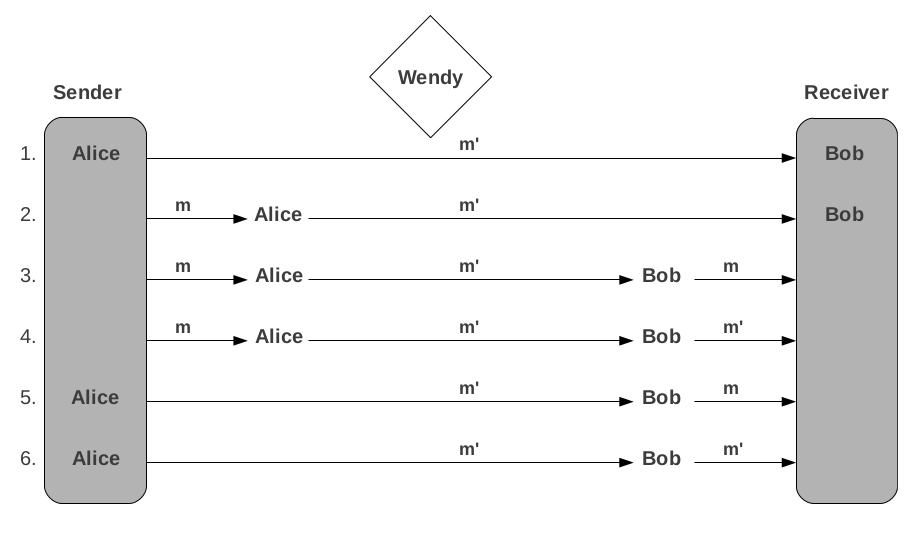
\includegraphics[width=0.8\textwidth]{communicationScenarios}
\caption{Communication Scenarios\cite{lewandowski}}
\label{fig:commScenarios}
\end{center}
\end{figure}

The six scenarios depicts different positions of Bob and Alice in the communication model, and the way the cover traffic (m) is manipulated by the covert channel (m\textprime).

The first scenario is the simplest one, it involves a communication between Bob and Alice, where Alice use directly the covert channel and insert the manipulated message, which is directed to Bob, the receiver. The remaining scenarios explores different combinations, depending on the behavior and identity of the sender, i.e. if Alice is the sender and introduces a manipulated message in the channel or Alice modifies an existing and legitimate one, or on the behavior and identity of the receiver, i.e. whether Bob is the receiver or, where he is not, if he restores or not the original message after reception.

``In these scenarios, Wendy always should be positioned between Alice and Bob so that she can monitor m\textprime\hspace{2pt} traffic. Were she positioned differently, and were unable to see m\textprime, her presence would be irrelevant to the covert communication''\cite{lewandowski}.

For the scope of this research, it is assumed that the sender can control the covert channel and insert directly the manipulated message. This reduction in scope, with respect to Lewandowski's study, is justified by the limitation in time, and by the simplicity of the network topology used for the experiment, which will be highlighted later in next chapters. However, it is worth saying that for an exhaustive testing of ICMPv6, related to covert channels, there are interesting implications to analyze inside the other scenarios, like the ability to preserve the covert channel in situations where Alice must modify the original message of the sender, or Bob must restore the original message before forwarding it to the legitimate receiver.

This assumption, however, has some implications:

``Alice can modify the traffic to a greater degree, since Bob does not necessarily expect the traffic to be meaningful and perhaps not even valid. On the other hand, if Alice and Bob use their own traffic to provide cover, they run a greater risk of exposure as they are openly communicating''\cite{lewandowski}. Furthermore, in this research, it is assumed that the sender and the receiver are different processes, but controlled by the same subject, the attacker.

Another topic to take into consideration, which relates to the behavior of the active warden, is the system and semantics preservation. The concepts have been applied first to preserve steganography \footnote{``The art or practice of concealing a message, image, or file within another message, image, or file'', \url{http://www.merriam-webster.com/dictionary/steganography}, accessed 24.3.2016}\cite{lucena2}, but ``the definitions can be applied to covert channels as well''\cite{lewandowski}.

In the context of covert channels, ``the property of syntax preservation determines whether the modified traffic m\textprime\hspace{2pt}adheres to the protocol syntax. On the other hand, the property of semantics preservation guarantees that the meaning of modified traffic m\textprime\hspace{2pt}is the same as the original traffic m, or in other words that covert channel communication performed by Alice and Bob does not alter the meaning of cover traffic''\cite{lewandowski}.

The above concepts acquire more relevance in a complex topology scheme, where an IPv6 packet must eventually traverse multiple wardens. Lewandowski's work defines the concept of ``location-based syntax and semantics preservation'', which is useful to differentiate between nodes, along the path, ``performing distinct functions'' and with ``multiple levels of protocol knowledge and understanding''. Each node, with a particular function in the network, may behave differently with respect to the packet in travel, and ``as a result, a modified traffic’s syntax or semantics might be deemed correct by an IPv6 node with limited protocol knowledge while at  the same time be rejected by a more knowledgeable node''\cite{lewandowski}.

This concepts will assume a particular relevance for this research when building the experiment. As it has been said before, it is important not only to understand the ICMPv6 protocol by itself, but also its relationship with devices like firewalls (the active warden) and the different configurations which produce different scenarios. Each configuration may lead to a different knowledge and understanding of the protocol by the node, which may affect the ability to preserve the covert channel, and must be taken into consideration. 

For example, it is worth to mention the reserved and unused fields, which are present in some message's headers. The receiver must ignore them, they have no meaning and any modification does not change the semantics. If the syntax is not altered, these fields may be ideal candidates for covert messages\cite{lewandowski}. Therefor, choosing a different configuration for the device, a firewall or router, may affect the level of knowledge of the protocol of that device, and the ability to preserve the covert channel. Or, in the other way, each scenario may produce different behaviors with the presence of a covert channel, and allow to assess a particular configuration and its ability to prevent it.

Indeed, ``the objective of covert channel participants is to conduct their communication in such way that the necessary modifications of the cover traffic are always syntax and semantics preserving \textit{with respect} to network nodes along the communication’s path''\cite{lewandowski}.

\textbf{Analyzed RFCs}\\

The following table (see~\ref{table:protocolsInScope}) shows the list of protocols and associated RFC from Lewandowski's study that are in scope with this research. 
\vspace{15pt}
\begin{savenotes}
\begin{table}[h]
\centering
\begin{tabular}{|C{8.5cm}|C{4.5cm}|}
\rowcolor{darkblue}
\hline
Protocol&RFC\\
\hline
\rowcolor{lightblue}
IPv6 \footnote{RFC2460 is only partially in scope with this research, but it is worth to mention it because in ICMPv6 specification there are frequently references to IPv6 fields, like source and destination addresses}&RFC2460\cite{rfc2460}\\
\hline
\rowcolor{lightblue}
ICMPv6&RFC4443\cite{rfc4443}\\
\hline
\rowcolor{lightblue}
Neighbor Discovery (ND) for IPv6&RFC4861\cite{rfc4861}\\
\hline
\end{tabular}
\caption{Investigated Protocols}
\label{table:protocolsInScope}
\end{table}
\end{savenotes}

\textbf{Properties of Covert Channels}\\

Lewandowski's study proposed six properties of covert channels which are important for the investigation. In this research, given its scope, two of them have been considered:
\vspace{-15pt}
\begin{enumerate}[noitemsep,topsep=0pt,partopsep=0pt]
 \item ``degree of packet alteration – syntax- and semantics-preservation level of altered packets''. Since each configuration can have different syntax- and semantics-preservation level, it is important to test each covert channel against each configuration, to assess both the warden configuration and the covert channel in this particular scenario\cite{lewandowski}.
 \item ``channel bandwidth – amount of data that can be transfered in given covert channel per packet of cover traffic''. This property does not affect the existence of the covert channel, but its ability to be preserved for a longer period. Depending on the bandwidth, a covert channel may be useful, from attacker perspective, only in situations with a low amount of data to be exfiltrated, or when it is possible to insert a delay in the transmission to avoid suspicion on the traffic\cite{lewandowski}.
\end{enumerate}

Lewandowski observed that some of the considered protocols, Neighbor Discovering is an example of them, ``are designed for operation on a single network segment. In consequence, any covert channel using these protocols as a cover will be similarly limited in its range'', and that ``the communication can be easily defeated by simple address-based filtering mechanism''\cite{lewandowski}.

This research, even though the observation may be correct, will not consider its assumption. The reason is given, as stated before, by the fact that it is important to consider also the actual transition period, where the two protocols, IPv4 and IPv6, coexist in many configurations. This scenario implies that both networks are in place, but the active warden is configured to inspect only IPv4-related protocols, thus with a low level of syntax and semantics preservation knowledge, and any IPv6 packet will transit without deep inspection. For the same reason, an address-based filtering mechanism for IPv6 would probably not be in place. Another aspect, still related to the active warden, is the direction of the communication, from the inside to the outside: since it is considered a communication from a trusted to an untrusted network, the default configuration may allow the traffic without restrictions.


\textbf{Analyzed Covert Channels}

In his research, Lewandowski defined a set of possible covert channels to test, which are spread among different protocols. For the scope of this research, only those that are mentioned in the aforementioned RFCs are taken into consideration.

Table~\ref{table:testedCC} summarizes the protocol or message, the fields, and the bandwidth of the tested covert channels.

\begin{savenotes}
\begin{table}[!htpb]
\centering
\begin{tabular}{|C{4.5cm}|C{3.0cm}|C{3.5cm}|C{3.0cm}|}
\rowcolor{darkblue}
\hline
Protocol/Message&Field&Covert Channel&Bandwidth\\
\hline
IPv6&Source Address&False Source Address&128 bits/packet\\
\hline
ICMPv6/All&Checksum&Arbitrary data&16 bits/packet\\
\hline
ICMPv6/Destination Unreachable&Unused&Arbitrary data&32 bits/packet\\
\hline
ICMPv6/Packet Too Big&Code&Undefined Code&8 bits/packet\\
\hline
ICMPv6/Packet Too Big&MTU&Arbitrary data&32 bits/packet\\
\hline
ICMPv6/Time Exceeded&Unused&Arbitrary data&32 bits/packet\\
\hline
ICMPv6/Parameter Problem&Pointer&Arbitrary data&32 bits/packet\\
\hline
ICMPv6/Echo Request&Code&Undefined Code&8 bits/packet\\
\hline
ICMPv6/Echo Request&Data&Arbitrary data&Unlimited\\
\hline
ICMPv6/Echo Reply&Code&Undefined Code&8 bits/packet\\
\hline
ICMPv6/Echo Reply&Data&Arbitrary data&Unlimited\\
\hline
\end{tabular}
\caption{Tested Covert Channels\cite{lewandowski}}
\label{table:testedCC}
\end{table}
\end{savenotes}

\textbf{Defense Against Covert Channels}

The first line of defense is the identification of a covert channel. Identification try to analyze the shared resource, i.e. header fields, during the design phase. Detection is the mechanism used to reveal an active covert channel. To detect and eliminate running covert channels it is possible to use protocol scrubbers, described in \cite{protocolScrubbers}, traffic normalizers, and the aforementioned active wardens. Protocol scrubbers and traffic normalizers try to find and eliminate ambiguities in the traffic flow. Active wardens and traffic normalizers analyze incoming traffic and modify outgoing packets based on their knowledge of the protocol, e.g. setting to zero reserved or unused fields. Active wardens have different level of knowledge, and abilities to detect and eliminate attacks, depending on the type, which can be stateless, stateful, and network-aware. Stateless wardens have no knowledge of previous traffic. Stateful wardens can detect flows of traffic and base its decision accordingly to preceding knowledge of the flow. Network-aware wardens have also the knowledge of the network topology. In case of ICMPv6, it is possible to limit covert channels by disabling some message types, or limiting the protocol size and rate\cite{milevaPanajotov}.

\subsubsection{Existing Tools}
\label{subsub:tools}

\textbf{cctool}

Lewandowski built a tool called \textit{cctool} in order to perform the tests. The tool has the ability to ``verify the existence of the covert channels, as well as to test the functionality of active wardens''. The results of his tests are strictly dependent on the quality of the wardens and on the scenarios used for the tests, which include, as mentioned before, also the possibility to modify the traffic in transit\cite{lewandowski}.

It is also worth mentioning some of the assumptions he made in order to better understand the tests. The syntax and semantics preservation are important factors in scenarios where the active wardens have the capabilities to understand, at different levels, the protocols. For example, Lewandowski built a scenario, called Cover Correctness Test, where a sender produces ICMPv6 traffic which is manipulated by Alice, but there is no receiver, namely Bob, at the end. The correctness of the covert channel, in this case, is demonstrated by the fact that an ICMPv6 Echo Request reaches the destination and an ICMPv6 Echo Reply is generated as usual. For such a test, ``the conclusion is that the covert message embedding by Alice does not disrupt the cover traffic enough to impede its normal functionality''\cite{lewandowski}.

One limitation of this kind of tests, as the author specified, is that many covert channel cannot be tested, in particular where an answer is not expected back.

Another type of scenario, instead, include also Bob, who is able to receive the message and restore it back to its initial, syntactically and semantically correct, version. In this case it is possible to test also messages which do not include an answer in its processing rule, because the test environment expected that ``both sender and receiver are located on a controlled network''\cite{lewandowski}.

The results performed by Lewandowski using cctool showed that the manipulation of the Source Address was defeated by the wardens. The tests on ICMPv6 implied an Echo Request, with correctness measured with the answer, resulted in a half of them defeated in the case of the manipulation of the Code field, while the covert channels were successful in case of the Data field manipulation.

One of the conclusions of Lewandowski study is ``that specification-based countermeasures cannot defeat some of the more sophisticated attacks''. In addition, with the tests performed with cctool, he demonstrated the existence of network storage covert channels in IPv6. Even though the test cases have not been exhaustive, his study has a great relevance for this research, in particular because of the accurate analysis and concepts underlined along the document\cite{lewandowski}.

\textbf{v00d00N3t}

Another interesting tool that have been built with the purpose to test covert channel in ICMPv6 is \textit{Voodonet}, or v00d00N3t. The purpose of the tool is to use ICMPv6 Echo messages as a covert channel to tunnel traffic. Covert Channel is embedded in the Data portion of Echo Reply message: the tool could send ``Echo Reply messages with a  payload of 1440 bytes in payload with no problem''. The capabilities of the tool is to send and receive data from keyboard (chat) or as text files. Another interesting functionality, which increases the ability to maintain the covert channel, is a time- or bytes-based mechanism to throttle the dispatch of the data\cite{voodoo}.

The two mentioned tools have been built mainly with testing purposes in mind. There is a suite of tools, instead, which has broadly functionalities and it is supposed to be used for penetration testing purposes: thc-ipv6.

\textbf{Thc-ipv6}

The thc-ipv6 attack toolkit\footnote{\url{https://www.thc.org/thc-ipv6/}, accessed 4.4.2016} is a ``complete tool set to attack the inherent protocol weaknesses of IPV6 and ICMP6, and includes an easy to use packet factory library''. The suite includes many features that could be used to test the IPv6 protocol in general, and the ICMPv6 protocol in particular\cite{thc}.

\textit{Alive6} is a tool used to check aliveness of IPv6 systems, both remotely using public addresses, and locally by taking advantage of an ICMPv6 Echo Request sent to the multicast addresses\cite{thc}.

\textit{Parasite6} can be used to perform a Man-in-the-middle attack to the internal LAN by exploiting the Neighbor Discovering process, and sending Neighbor Advertisements to nodes with the attacker MAC address and the IPv6 address of the requested node\cite{thc}.

Another interesting tool is \textit{redir6}, which use ICMPv6 redirect messages. The proposed technique is to take advantage of the Redirect Header as an option for the Redirect message, which includes the IPv6 header and the data\cite{thc}:
\vspace{-15pt}
\begin{enumerate}[noitemsep,topsep=0pt,partopsep=0pt]
 \item Attacker sends an Echo Request with the target address as Source Address and the victim address as Destination Address.
 \item The victim receive the Echo Request and sends an Echo Reply to the target (which can be intercepted by the attacker)
 \item Attacker crafts a Redirect message, using the previous Echo Reply in the Redirect Header option, with local router as Source Address, victim as Destination Address, and attacker as Target Address
\end{enumerate}

It is interesting to highlight that the cited paper, dated 2006, took into account the transition scenario and emphasized the possibility to attack the dual stack if proper filtering were not in place for both IPv4 and IPv6.


\subsection{Other Projects}
\label{sub:otherProj}

\subsubsection{IPv6 Ready}
\label{subsub:ipv6Ready}

The IPv6 Ready Logo \footnote{\url{https://www.ipv6ready.org}, accessed 2.3.2016} is ``a conformance and interoperability testing program intended to increase user confidence by demonstrating that IPv6 is available now and is ready to be used''. Its mission `` is to define the test specifications for IPv6 conformance and interoperability testing, to provide access to self-test tools and to deliver the IPv6 Ready Logo'' \cite{ipv6ready}.

The project is composed by an Administrative Group, responsible for the administration, the definition of procedures and regulations, and by a Technical Group, which is responsible to define the tests specifications and submit them to the Administrative Group in order to be published for public review.

The procedure to obtain the certification and the possibility to exhibit the IPv6 Ready Logo on the products is to first download the test specifications. After that it is possible to use a self-testing tool or to submit the product to specialized and approved laboratories.

IPv6 Ready project entered the phase 2 and version 4.06 of the test since 2010. Phase 1 indicated ``that the product includes IPv6 mandatory core protocols and can interoperate with other IPv6 equipments'', while Phase 2 indicated ``that a product has successfully satisfied strong requirements stated by the Logo Committee''.

The project produced a detailed set of documents\cite{ipv6readyCore}\cite{ipv6readyCore2} which indicate the required network topology, as well as the detailed list of test to be performed against each protocol. Test are organized in sections based on RFCs, and inside each sections in groups defined by their functionalities, e.g. Address Resolution and Neighbor Unreachability Detection for the section RFC 4861. Inside the section it is defined the scope, which describes broadly the content of the RFC, and the default packet of the message type (ICMPv6). The following table(see~\ref{table:ipv6readyPacketEx}) is an example of a default Router Advertisement packet:

\begin{savenotes}
\begin{table}[h]
\centering
\begin{tabular}{|C{3.0cm}|C{4.0cm}|C{5.0cm}|}
\rowcolor{darkblue}
\hline
Header&Field&Value\\
\hline
\multirow{3}{*}{IPv6 Header}&Source Address&TR\footnote{Testing Router} Link-Local address\\ \cline{2-3}
&Destination Address&All-nodes multicast address\\ \cline{2-3}
&Next Header&58\\
\hline
\multirow{7}{*}{ICMPv6 Header}&Type&134\\ \cline{2-3}
&Code&0\\ \cline{2-3}
&M Bit&0\\ \cline{2-3}
&O Bit&0\\ \cline{2-3}
&Router Lifetime&20s\\ \cline{2-3}
&Reachable Time&10s\\ \cline{2-3}
&Retrans Timer&1s\\
\hline
\multirow{5}{*}{Prefix Option}&Type&3\\ \cline{2-3}
&L Bit&1\\ \cline{2-3}
&A Bit&1\\ \cline{2-3}
&Valid Lifetime&20s\\ \cline{2-3}
&Preferred Lifetime&20s\\
\hline
\end{tabular}
\caption{Router Advertisement Packet example for IPv6 Ready Project}
\label{table:ipv6readyPacketEx}
\end{table}
\end{savenotes}


In each group, e.g. ``Address Resolution and Neighbor Unreachability Detection'', the tests are described with a purpose, e.g. ``Verify that a node correctly determines that a destination is on-link'', the references inside the specifics RFCs, and the test setup with each packet definition, with the fields that differ from the mentioned default packet setup. Then the procedure to perform the test is shown, divided in parts. An example of that is the following:

\textit{Part A: Link-local Address}:
\vspace{-15pt}
\begin{enumerate}[noitemsep,topsep=0pt,partopsep=0pt]
 \item TN1\footnote{Testing Node 1} transmits Packet A an Echo Request with TN1’s link-local source address.
 \item Observe the packets transmitted by the NUT\footnote{Node Under Test}.
\end{enumerate}

which is followed by the ``Observable Results'':

\textit{Part A}:
\vspace{-15pt}
\begin{enumerate}[noitemsep,topsep=0pt,partopsep=0pt]
 \item[2] The NUT should send a Neighbor Solicitation with Target Address equal to TN1’s link-local address, indicating that the NUT has successfully determined that TN1 was on-link.
\end{enumerate}


The project covers all the RFCs in scope with this research with extensive tests, with great emphasis on RFC 4861, which is divided in three groups:
\vspace{-15pt}
\begin{enumerate}[noitemsep,topsep=0pt,partopsep=0pt]
 \item Address Resolution and Neighbor Unreachability Detection
 \item Router and Prefix Discovery
 \item Redirect Function
\end{enumerate}

Tests cover the expected functionality, specified by the RFC, but also the behavior of nodes in case of manipulation of the messages, e.g. a wrong code field.

From the perspective of this research the test quality is very good, and it covers many possibilities to attempt to gain a foothold from the outside to the inside network. One missing part is the assessment of the opposite direction, from the inside to the outside, as is the case in presence of possible cover channels. The lack of references about the configuration of the wardens prevents the assessment of this kind of attacks, specifically with regards to the syntax and semantic preservation knowledge of the warden.

Another issue that it is worth to underline is that the project assumes an IPv6 world, without considering the transition scenario. This is not a critique towards the project, which aim is to test the readiness of devices and implementations with regard to IPv6, but only a consideration that limits the scope of the project towards this research.


\subsection{Summary}

Inside this section, this research started to analyze the background, that is RFCs document. RFCs are documents developed as an agreement to define standards upon which the Internet is built. The two main documents which are in scope with the research are RFC 4443 and RFC 4861, which define the ICMPv6 messages format and the processes for which they have been developed. Besides the header formats, RFCs include directives to the protocol implementation, using terms like MUST and SHOULD. This research examined the messages and presented them with a brief description. The actual header representations of each message are left to Appendix 1. Inside Appendix 2, it is possible to see the ICMPv6 specifications, with a selection of the specification and the term that the RFC uses to specify which feature is mandatory (MUST) or it is better to have. These specifications will also put together the tests selected for the experiment.

After the background analysis, this research started to examine the concept of Covert Channels, which is a ``communication paths that allow information transfer in violation of a system’s security policies''. This is the first step on analyzing both directions of the network traffic flow, from the inside and trusted network to the outside. Even though a covert channel may exist in both directions, it is useful to understand, for example in case of APT, that an attacker may already have a foothold in the network and want to exfiltrate sensible data to an outside address. In this context it is important to consider the presence of wardens, firewall or routers, that may disrupt the covert channel. For such a reason, during the experiment, will be noteworthy to consider different scenarios based on different warden configurations.

The research continue by presenting the existing tools. Two of them, cctool and v00d00N3t, have been built to test the covert channels. The third is a suite of tools, or toolkit, which has been thought to perform security tests on IPv6 and ICMPv6.

After that, the IPv6 Ready project has been presented. The project's aim is to evaluate the readiness of the different products to IPv6 with an extensive set of tests based on the RFC specifications. The project offers, in many aspects, to analyze the opposite network flow direction with respect to covert channels, from the outside to the inside network.

In order to conclude this chapter, it is noteworthy to say that all the documents so far presented are, with different degrees, relevant for this research. The RFCs establish the base of the research, while the other documents offer an insight to understand the contest of some attacks and the reasons behind the choice to perform the tests. Besides those, other documents have been examined, but have been considered not relevant. Example are documents related to the common attacks on ICMPv6 and enumeration\cite{sans}, RFCs related to the internal network only and not defining new messages\cite{rfc4862}, or related to internal Denial of Service 
attacks\cite{smurf}.



\pagebreak

%------------------------------METHODOLOGY-----------------------------------
\section{Methodology}
\label{sec:3}

The second chapter of this research starts by analyzing the background. The analyzed RFCs define the type of messages that compose the ICMPv6 protocol. For each message the RFCs specify the header and the fields, and the behavior of the protocol to fulfill its functions. The specifications include how to validate a message, the mandatory and optional fields, the data that each field must, should, or may deliver. The language use the terms must, should, may in order to underline what is mandatory to include in the implementation of the protocol, what it is better to include, and what may or not be implemented, leaving the developer more freedom in how to implement a task. The RFCs represents the knowledge about the protocol. The observation of the rules could lead to think if it is possible to break the rules in some way, and what could happen if different implementors interpret them in a different way.

Another observation regard the environment on which the protocol operate: a network based on a specific protocol suite. The Internet is a complex environment composed by devices interconnecting each other, using many protocols. This complexity make the Internet an environment not suitable to try to find an answer to the questions derived by the observation. This is because the amount of variables that it introduces do not allow to derive a unique consequence from an action, and thus reliable conclusions. In order to be able to derive reliable conclusions the environment must be simplified and be controllable. A controlled procedure needs to have exactly one variable, and to achieve that, as it has been mentioned before, a particular configuration must be defined. A specific configuration of the environment represents a constant, thus allowing to modify a specific rule. A set of tests is performed using manipulated rules against a well defined configuration. Then the same set of test can be performed against another configuration, leading to a number of tests equal to the number of configurations multiplied by the number of elements in the set.\cite{secExperiments}

After the process of observing the background, and the environment in which the ICMPv6 protocol operate, this research found that the best methodology to follow is the scientific method. The reason behind the choice is that many element of the analysis of the second chapter, the observation of the data, led to the formulation of questions and hypothesis, that could be validate, or negate, by experimentation. As it will be better explained next, the process of the scientific method is ideal to test the hypothesis derived by the research questions, taking into account the different configurations of the environment which has been discussed in the second chapter.

\subsection{Scientific Method}
\label{sub:sciMeth}

The scientific method has its roots in the ancient Greek philosophy, with Plato and Aristotle. The human reasoning has been the basis for the scientific evolution and studies, with the expression of an hypothesis, the argumentation about the truth or untruth, and eventually the formulation of a theory. Many centuries later, with the Enlightenment, two ways of looking at science coexisted in the developing scientific community: rationalism and empiricism. While the former accepted the human intuition, mainly in the field of natural science, and then applies testing hypothesis in order to formulate theories, the latter was more based on the observation of the data and then experimentation. Since then, both approaches have influenced the developing of the scientific method and reasoning, and applied to natural and human science.\cite{carroll}

Another important distinction is between quantitative and qualitative research. Quantitative research is based on the use of statistics or on data that are quantifiable and measurable, in order to produce a result which is not biased on some context and, thus, could lead to a generalization of some theories. Qualitative research, instead, introduces the contextualization and relies on the context in which it is possible to observe a given phenomenon, which is more related to the human science, where observation and definition of a context in which human beings interact may allow to validate or not an hypothesis.\cite{kaplan}

This research uses both a quantitative and qualitative approach to perform the experiment. The qualitative approach is necessary to set up the experiment because of two factors: the choice of the tests and the considerations about the context. The tests are chosen starting from the description of the protocol inside the RFCs, which are for their nature not representable in a mathematical way. Among all the possible tests, some of them are considered for the experiment, as it will presented later. The context is also very important and it involves the observation of human behavior in the configuration of the border network devices and the choices of the implementers of the end devices. The quantitative approach arises after the definition of the test set. Each test is performed against a well defined configuration. The set of tests and a specific configuration is an experiment where the only variable is the test itself, and the validation or not of the hypothesis can be done only for that specific configuration. In this way, this research is considering the quantitative approach, because inside the experiment, after its set up, no other variable other then the specific test will change, thus allowing it to be measurable in a binary way: either failed or succeed. The conclusions of the experiments, however, because of its context-dependent nature, could not lead to the formulation of a mathematical evaluation. In other words it wont be possible to state that the ICMPv6 protocol is vulnerable by itself, but only that, given this specific configuration, the protocol introduces some vulnerabilities.

Following the work of Peisert and Bishop in \textit{How to Design Computer Security Experiments}, this research defines the following steps:
\vspace{-10pt}
\begin{enumerate}[noitemsep,topsep=0pt,partopsep=0pt]
 \item Form hypothesis
 \item Perform experiment and collect data
 \item Analyze data
 \item Interpret data and draw conclusions
\end{enumerate}

In addition to the aforementioned steps, Peisert and Bishop define three qualities, the most relevant in the domain of computer security, that the procedures requires. The procedures must be falsifiable, which means that the experiment must not be set up in order to justify a positive answer, but to test hypothesis that may ends up to be false. The procedures must be controlled, which involves the presence of exactly one variable. The procedures must be reproducible, which assumes that it is possible to repeat the experiment and obtain the same result.\cite{secExperiments}

\subsection{Research Questions and Hypothesis}
\label{sub:reearchQandH}

The research questions are the starting point in order to define the hypothesis. Research questions express what the research want to know about the specific topic, and leads to definition of an hypothesis, which represents what the researcher want to validate (or invalidate) through the experiments. This research starts with a general research question, from which two additional and more specific research questions have been derived.

\subsubsection{Research Question}
\label{subsub:researchQ}

\textit{Is it possible to manipulate the ICMPv6 protocol and, by traversing border network devices, use in an unauthorized way a remote network?}

This question is a generalization which broadly introduces what this research want to know and test in relationship with the ICMPv6 protocol. Since the question introduces too many variables, it is useful and necessary to narrow down the scope, by defining two more specific research questions.
\begin{enumerate}
 \item \textit{Is it possible to exfiltrate data without authorization, from an internal network to the outside, traversing a border network device, by manipulating the ICMPv6 protocol?}
 \item \textit{Is it possible to gain unauthorized access to an internal network, from the outside and traversing a border network device, by manipulating the ICMPv6 protocol?}
\end{enumerate}

\subsubsection{Hypothesis}
\label{subsub:hypothesis}

The formulation of the hypothesis follows the research questions. The hypothesis is the statement that the experiment aims to validate, which, following the aforementioned qualities of the process, may be negated by the experiment itself and by the following interpretation of data and conclusions.

The hypothesis of this research is:

\textit{It is possible to manipulate the ICMPv6 protocol to use a remote network in an unauthorized way, after traversing a border network device}

Even thought this research will prove the truth of this hypothesis, some clarifications are necessary, and the final discussion inside the conclusions will take them into account. The first consideration is related to the general hypothesis itself, which, given its generality, may be less interesting from a scientific point of view. As stated before, each test and configuration is an experiment that may lead to prove the truth of the hypothesis for this exact experiment. The truth is related to a single experiment in the context of a general hypothesis, and the more experiments evaluate to true, the more relevant will be the results. It is very important to emphasize and understand that once a single experiment evaluate to true, the general hypothesis will be proved to be true. In other words, the truth of the hypothesis is the result of the logical \textit{or} of the set of tests performed against each configuration. From this point of view the two more specific research questions, and the two sub-hypothesis, are more relevant because by narrowing down the problem, they define more specifically the context and give more indication about the results. The two sub-hypothesis are:
\begin{enumerate}[ref=Hypothesis \arabic*]
 \item \label{firstHyp} \textit{It is possible to manipulate the ICMPv6 protocol to exfiltrate data without authorization from an internal network to the outside and traversing a border network device}
 \item \label{secondHyp}\textit{It is possible to manipulate the ICMPv6 protocol in order to traverse a border network device and gain unauthorized access to an internal network}
\end{enumerate}

The keywords of the first hypothesis are \textit{exfiltrate data without authorization}. While the meaning of the first hypothesis is clear, the second one may be confusing. The keywords of the second hypothesis are \textit{gain unauthorized access}. With gaining unauthorized access, this research do not refer only to the action of controlling a device remotely, but includes also the access to a process to stop it from working (i.e. denial of service) and the access to a process to change its behavior (i.e. man in the middle).

The assumption done before, that is, that the truth of the hypothesis is given by the logical \textit{or} of the set of tests performed against each configuration, acquires more relevance in the case of one of the sub-hypothesis, because a more thorough specification of the problem has been made.

As it will be discussed in the conclusions, the relevance of the results is an important topic. This is because the aim of this research is not only to prove the truth or untruth of the hypothesis, but also to evaluate the impact that the exploitation of a vulnerability could have on an organization in relationship to the chosen wardens, the border network devices, and the deployed configuration.

\subsection{Experiment Foundation}
\label{sub:expFound}

As shown before, the first step of the scientific method involves the definition of the research question, which in this case led to two sub-questions, and the formulation of the hypothesis and sub-hypothesis. The next step involves the execution of the experiment. This research will describe the experiment implementation in detail during next chapter and its execution afterwards. Before that, it is important to discuss the foundation of the experiment, that is, the choices and reasons behind it.

The selection of the test set is a critical task because it is the input of the experiment.

\subsubsection{Test set selection}
\label{subsub:testSel}

``[T]he truth or falsity of every hypothesis is to some extent conditioned on the input data set [...] an additional step in testing a hypothesis is the validation of the input data set''\cite{secExperiments}. The statement underlines the importance of the test set selection discussed in this section.

Inside chapter two (see~\ref{sec:2}), this research analyzed two RFCs which describe the ICMPv6 protocol and its messages. The analysis had the purpose to show the background of this research and to underline the basis to select the test set for the experiment. The background analysis produced a set of tables (see~\ref{Appendix 1} and~\ref{Appendix 2}). 

In \ref{Appendix 1} it is possible to see the header of the messages with its fields. In the context of the set of tests, the fields acquire relevance to prove the truth of the first hypothesis, that is, the use of ICMPv6 to exfiltrate data from an internal network. Each field, with few exceptions, has been designed to carry data to fulfill a specification of the protocol. In the case of the data exfiltration described in this research, where the attacker controls both processes of sending and receiving data, only the border network device may perform some checks to validate the compliance with the protocol. The protocol itself may be used just as a transport vector for some data, by means of its fields, with the exception of the destination address specified in the IPv6 protocol, which is necessary to forward the packet to its destination. The aforementioned few exceptions are the unused or reserved fields, when defined by the message, which have no specific purposes in the context of the functionality of the protocol. In addition, each field shows an important indication for the purpose of exfiltrating data, the bandwidth. In fact, depending on the size of the field and of the data to be exfiltrated, it is possible to predict beforehand how many packets the process will use. This research, during the experiment, manipulates each ICMPv6 field and options headers against each border network device configuration, in order to test the hypothesis and assess the behavior of the warden.

In \ref{Appendix 2}, the tables show the specifications of each ICMPv6 message and the processing rules in terms of what must, should, or may be implemented. These specifications and processing rules define the behavior of the protocol in relationship with the functions for which it is used by other processes or protocols. Even though some of the specifications refers to an header field, as it has been mentioned above, the reasons behind the base used to choose the set of test in this appendix is different. While to test the first hypothesis both the sending and receiving processes are controlled by the attacker, the second hypothesis implies that the attacker controls only the sending process. In fact, if a packet successfully traverse the border network device, it is the behavior of the protocol and the implementation of the end device, i.e. the receiving process, to be under testing. In other words, it is the ending device that determines the truth of the hypothesis in case a packet has been able to reach it. In such a situation the it is useful to consider the specifications that include the terms must, should, and may. This research assumes that at least the specifications including a must have been implemented. Nevertheless, each implementation may differ from another one by a very small degree, therefor such specifications must be included in the set of tests. The same applies to specifications characterized by the terms should and may, which, in addition, do not have the mandatory nature of the musts. 

Another important aspect that has been taken into consideration in the choice of the set is the necessity to avoid the introduction of additional variables that it is not possible to control and verify in a reproducible way. An example of that is the last specification included in table \ref{table:4443ProcRules}, which specifies the need to limit the transmission rate of ICMPv6 error messages to limit the bandwidth and forwarding costs. Even though an high transmission rate may lead to a denial of service, there are other variables that affect the test of the specification, like the type of physical connection or the bandwidth usage of other processes. Therefor this type of specifications have not been selected.

The next step is the experiment environment and the reasons behind the choices.

\subsubsection{Environment}
\label{subsub:enviroment}

The environment has been chosen taking into account the possibility to test the hypothesis and properties related to the methodology. To test the hypothesis, the experiment must include an attacking machine positioned in an outside network, which border is delimited by a border network device. The attacking machine is responsible for the receiving process in testing the first hypothesis (see~\ref{firstHyp}), and it is used to send the manipulated ICMPv6 packets in testing the second hypothesis (see~\ref{secondHyp}). The network topology includes two wardens, a dedicated Cisco Adaptive Security Appliance (ASA)\footnote{\url{http://www.cisco.com/c/en/us/support/security/asa-5505-adaptive-security-appliance/model.html}}, and a Linux host with firewall (i.e. iptables) capabilities. Each experiment uses only a warden with a specific configuration. The details of each configuration is discussed in the next chapter (see~\ref{sec:4}). The environment includes two end devices, one Linux host and one windows host. End devices purpose is to be responsible for the sending process in testing the first hypothesis (the Linux host), and, when testing the second hypothesis, to receive the ICMPv6 manipulated packets.

The choice of the devices for the experiment has been made taking into account the availability of the devices or virtualized environments. For virtualized environments, one limitation was the available memory (8GB) on the laptop used to develop the attacking framework and to host the virtual machines. The first research about the environment aimed to have a complete virtualized environment. The difficulties in that research arose in finding a virtualized environment for one of the warden, because one of the objectives of this work is to test a security device which may be used in production systems, like a Cisco firewall. Since there are no freely available images, this possibility has been abandoned. After a bit of research, it has been possible to obtain a physical device (ASA firewall) on University's laboratory, which also has the advantage to decrease the overall need of memory for the virtualization. The virtualized environment is built on top of VirtualBox\footnote{\url{https://www.virtualbox.org/}}, chosen because it is available as open source software with GNU General Public License (GPL) version 2\footnote{\url{http://www.gnu.org/licenses/old-licenses/gpl-2.0.html}}, and supports for many guest operating systems. The second warden is a Debian Jesse\footnote{\url{https://www.debian.org/releases/jessie/}} Linux virtualized guest, which uses iptables\footnote{\url{https://wiki.debian.org/iptables}} to provide firewall services. The virtualized environment has been chosen also for the two end devices, a Debian Jesse guest OS and a Windows 7 guest OS. In this case Debian Jesse has been chosen because it is a Linux open source OS, and because a Linux-based machine could be used as a server in production environments. The Windows 7 guest, instead, may represent common workstations in an internal network, and a virtual image could be downloaded\footnote{\url{https://developer.microsoft.com/en-us/microsoft-edge/tools/vms/windows/}} with a free trial license. The last device to consider is the attacking device, which had a constraint: because of the physical firewall, also that machine must be a physical device to form a network segment with the firewall. This constraint at the beginning posed some issues, because of a limited availability of devices. After some research the choice has fallen on a Raspberry Pi\footnote{\url{https://www.raspberrypi.org/}} with a Kali Linux OS. The reasons behind this choice is both on Kali Linux and Raspberry Pi as a attacking/pentesting device. Kali Linux has support for Raspberry Pi, and it is possible to download a pre-built image from Offensive Security website\footnote{\url{https://www.offensive-security.com/kali-linux-arm-images/}}, which are the creators of Kali. In addition, Raspberry Pi with Kali Linux may be a choice for attackers as a portable hacking station. Its dimension may allow to hide it or to use it without causing suspicion in places where the use of a laptop is not common.


\subsubsection{Border Network Device Configurations}
\label{subsub:borderConfig}

The firewall device, or service, is a key point in the security of the internal network of an organization. The market offers the state-of-the-art products, which include high performances in terms of forwarding capabilities, processing power, deep content inspection, services. Nevertheless, what make a firewall a security device that protect an internal network is the configuration. Most of the products include a default configuration, which must be perceived as a base, a starting point that should be tuned to the requirements of the organization. The default configuration may be enough to cope with the most common attacks, but from an attacker point of view it is sufficient to discover just one entry point in order to pass through. This is even more effective considering an APT.

The hypothesis of this research includes a firewall, as a border network device, because of the belief that the better way to test the ICMPv6 protocol is by correlating the implementation in end devices with the configuration of the firewall. Of course, each protocol may be vulnerable by itself, because of both its design or implementation, and dedicated research must be done as well. Nevertheless, there are scenarios in which, even if the exploitation of a vulnerability is possible, the surrounding environment may be a challenge for an attacker, reducing the likelihood to reach his goals.

Each firewall configuration represents a scenario, and an experiment, in which there is a set of tests and an end device. The set of configurations considered for this research is not exhaustive. The reason is that, even though there are best practices, each configuration must be fine-tuned for a particular set of requirements. The intent of this research is to show what may be the choice of different actors, based on different budgets.

A Linux-based machine, with firewall services, may be the choice of an organization with a low budget. Instead, a company with more resources may choose a dedicated device. This broad category includes organizations without security specialists, which use the default configuration, or companies with the needed expertise to follow best practices. 

In order to deploy meaningful configurations for the experiment, this research examined documents, best practices and RFCs. 

The first document has been written by the National Institute of Standards and Technology (NIST)\footnote{\url{http://www.nist.gov/}}, which has a dedicated chapter on firewall policy and a sub-chapter on IPv6. Inside the section there is a statement that shows how much has to be done for IPv6 and ICMPv6, which says ``[b]ecause IPv6 deployment is still in its early stages, there is not yet widespread agreement in the IPv6 operations community about what an IPv6 firewall should do that is different from IPv4 firewalls''. The suggestions inside the document are more related to filtering packets with an invalid source or destination addresses, for example a link local address arriving at the boundary from the outside network. Another advice is to block all IPv6 traffic in the case that the organization do not use IPv6. For what is related to ICMP6, the document suggested to refer to RFC 4890, which will be examined next in this chapter.\cite{nist}

The second document have been draft by the National Aeronautics and Space Administration (NASA)\footnote{\url{http://www.nasa.gov/}} by means of the Communications Service Office (CSO), and used for the NASA Integrated Communication Services (NICS) contract\footnote{\url{https://cso.nasa.gov/content/about-cso-and-nics}}. The documents describes best practices related to IPv6 in detail. The relevance for this research is limited, because the document refers mostly to internal networks. Specifically, in the chapter related to firewall rules, the document warns about the need of neighbor solicitation and advertisement messages in order for the Neighbor Discovery protocol to work\cite{nics}.

The most important suggestions for this research are described in RFC 4890. Chapter 4 divides firewall rules in 5 broad categories:
\vspace{-15pt}
\begin{enumerate}[noitemsep,topsep=0pt,partopsep=0pt]
 \item Messages that must not be dropped
 \item Messages that should not be dropped
 \item Messages that may be dropped in firewall/routers
 \item Messages that administrators may or may not want to drop depending on local policy
 \item Messages that administrators should consider dropping
\end{enumerate}
Inside each category the RFC defines ICMPv6 messages that belongs to it, which in fact allows to build firewall rules accordingly\cite{rfc4890}.

The last source is related to the configuration of a Linux-based host with firewall services. The source also refers to RFC 4890, but as the author states, do not cover all the advices from there. Nevertheless this is a very good starting point to implement the Linux-based scenario of this research\cite{ip6tablesGiobbi}. In addition, there is a basic script\footnote{\url{http://www.cert.org/downloads/IPv6/ip6tables_rules.txt}, accessed 22.4.2016} that is downloadable from the main Computer Emergency Response Team (CERT) website, hosted by the Carnegie Mellon University\footnote{\url{http://www.cmu.edu/}}. 

Based on the above described information, this research decided to implement the following configuration categories:
\vspace{-10pt}
\begin{enumerate}[noitemsep,topsep=0pt,partopsep=0pt]
 \item Linux-based firewall services using ip6tables\footnote{\url{http://ipset.netfilter.org/ip6tables.man.html}}
 \item Cisco ASA firewall with default configuration (without IPv6 filtering)
 \item Cisco ASA firewall with default configuration (no native IPv6, complete IPv6 filtering)
 \item Cisco ASA firewall with RFC 4890 best practices
\end{enumerate}


\subsubsection{Testing/Attacking framework}
\label{subsub:framework}

The experiment part of this research includes a framework which is able to manipulate and send ICMPv6 packets to test the hypothesis. The framework is written in Python\footnote{\url{https://www.python.org/}} as a programming language, which use an external library to manipulate ICMPv6 messages, called Scapy\footnote{\url{http://www.secdev.org/projects/scapy/}}.

Python is a programming language which is possible to use in scripts, with functions, and with object oriented programming. It is installed by default in most Linux distributions and allows to use many third party libraries related to computer security and network testing. Example of that is a project supported by Open Web Application Security Project (OWASP)\footnote{\url{https://www.owasp.org/index.php/Main_Page}}, called OWASP Python Security Project\footnote{\url{http://www.pythonsecurity.org/}}.

Scapy is a very flexible tool that allows to build packets for many protocols. It allows to use the default protocol implementation, but it is also possible to manipulate packets or create new protocol from scratch. In addition, it allows to control the process of sending and receiving packets, and to visualize the content in different formats in order to build detailed reports. For these reasons, it the ideal tool to build a framework for the experiment.

\subsection{Summary}
\label{sub:methConclusions}

This research started this section by presenting the methodology, which is based on the scientific method. After a brief historical introduction, there is a description of the steps that the scientific method involves, starting from the research questions, which form the basis for the hypothesis, then going through the experiment, the analysis of the data, and finally the interpretation and conclusions.

After the general introduction of the methodology, this chapter went through the definition of the hypothesis that have to be tested during the experiment. The general hypothesis produced two more specific hypothesis, which are in relationship with the traffic flow direction of the ICMPv6 packets, from the internal network to the outside, and from the outside to the internal network, both of them traversing a firewall.

The next step in the chapter has been to describe the foundation of the experiment. This research first defined the reasons behind the choice of the test set for each hypothesis. The environment is another important aspect, with the choice of the involved devices which, sometimes, has been conditioned by the available resources.

The configuration of the firewall, as border network device, is another important topic, because each configuration represents a scenario. A scenario is a representation of what might be the choice of an organization for a firewall, based on aspects like the available budget, or the needed expertise to configure it.

Finally, this chapter introduced the components used to build the testing/attacking framework, which are python as a programming language and scapy as packets manipulating library.

The next chapter will dig deeper in the implementation of the experiment, with the details of each involved component.




\pagebreak

%------------------------------IMPLEMENTATION-----------------------------------
\section{Implementation}
\label{sec:4}

\pagebreak

%------------------------------EXPERIMENT-----------------------------------
\section{Experiment}
\label{sec:5}

\pagebreak

%------------------------------RESULTS-----------------------------------
\section{Results}
\label{sec:6}

\pagebreak

%------------------------------CONCLUSIONS-----------------------------------
\section{Conclusions}
\label{sec:7}

\pagebreak

%------------------------------REFERENCES-----------------------------------

\addcontentsline{toc}{section}{References}


\bibliographystyle{IEEEtran}
\bibliography{bibi.bib}


\pagebreak

%-----------------------------APPENDIX--------------------------------

\appendix

\section{Appendix 1 - Protocol Headers}
\label{Appendix 1}
%\addcontentsline{toc}{section}{Appendix 1}

\subsection*{IPv6}

\begin{savenotes}
\begin{table}[!htpb]
\centering
\begin{tabular}{|C{40pt}C{40pt}C{40pt}C{40pt}C{40pt}C{40pt}C{40pt}C{40pt}|}
\hline
\multicolumn{1}{|C{40pt}}{\cellcolor{darkblue} Version}&\multicolumn{2}{|C{80pt}|}{\cellcolor{lightblue} Traffic Class}&\multicolumn{5}{C{200pt}|}{\cellcolor{darkblue} Flow Label}\\
\hline
\multicolumn{4}{|C{160pt}}{\cellcolor{lightblue} Payload Length}&\multicolumn{2}{|C{80pt}|}{\cellcolor{darkblue} Next Header}&\multicolumn{2}{C{80pt}|}{\cellcolor{lightblue} Hop Limit}\\
\hline
\rowcolor{darkblue}
\multicolumn{8}{|c|}{}\\
\rowcolor{darkblue}
\multicolumn{8}{|c|}{}\\
\rowcolor{darkblue}
\multicolumn{8}{|c|}{}\\
\rowcolor{darkblue}
\multicolumn{8}{|c|}{\multirow{-4}{*}{\hfil Source Address}}\\
\hline
\rowcolor{lightblue}
\multicolumn{8}{|c|}{}\\
\rowcolor{lightblue}
\multicolumn{8}{|c|}{}\\
\rowcolor{lightblue}
\multicolumn{8}{|c|}{}\\
\rowcolor{lightblue}
\multicolumn{8}{|c|}{\multirow{-4}{*}{\hfil Destination Address}}\\
\hline
\end{tabular}
\caption{IPv6 Header}
\label{table:IPv6}
\end{table}
\end{savenotes}

\subsection*{ICMPv6}

\subsubsection*{RFC 4443}

The following are the Protocol Headers described in RFC 4443.\\

\vspace{15pt}
\textbf{Destination Unreachable}
\begin{savenotes}
\begin{table} [!htpb]
\centering
\begin{tabular}{|C{40pt}C{40pt}C{40pt}C{40pt}C{40pt}C{40pt}C{40pt}C{40pt}|}
\hline
\multicolumn{2}{|C{80pt}}{\cellcolor{darkblue} Type}&\multicolumn{2}{|C{80pt}|}{\cellcolor{lightblue} Code}&\multicolumn{4}{C{160pt}|}{\cellcolor{darkblue} Checksum}\\
\hline
\rowcolor{lightblue}
\multicolumn{8}{|c|}{Unused}\\
\hline
\rowcolor{darkblue}
\multicolumn{8}{|c|}{}\\
\rowcolor{darkblue}
\multicolumn{8}{:c:}{\multirow{-2}{*}{\parbox{10cm}{As much of invocking packet as possible without the ICMPv6 packet exceeding the minimum IPv6 MTU}}}\\
\hdashline
\end{tabular}
\caption{Destination Unreachable}
\label{table:destUnreach}
\end{table}
\end{savenotes}

\textbf{Packet Too Big}
\begin{savenotes}
\begin{table}[!htpb]
\centering
\begin{tabular}{|C{40pt}C{40pt}C{40pt}C{40pt}C{40pt}C{40pt}C{40pt}C{40pt}|}
\hline
\multicolumn{2}{|C{80pt}}{\cellcolor{darkblue} Type}&\multicolumn{2}{|C{80pt}|}{\cellcolor{lightblue} Code}&\multicolumn{4}{C{160pt}|}{\cellcolor{darkblue} Checksum}\\
\hline
\rowcolor{lightblue}
\multicolumn{8}{|c|}{MTU}\\
\hline
\rowcolor{darkblue}
\multicolumn{8}{|c|}{}\\
\rowcolor{darkblue}
\multicolumn{8}{:c:}{\multirow{-2}{*}{\parbox{10cm}{As much of invocking packet as possible without the ICMPv6 packet exceeding the minimum IPv6 MTU}}}\\
\hdashline
\end{tabular}
\caption{Packet Too Big}
\label{table:packettoobig}
\end{table}
\end{savenotes}

\textbf{Time Exceeded}
\begin{savenotes}
\begin{table}[!htpb]
\centering
\begin{tabular}{|C{40pt}C{40pt}C{40pt}C{40pt}C{40pt}C{40pt}C{40pt}C{40pt}|}
\hline
\multicolumn{2}{|C{80pt}}{\cellcolor{darkblue} Type}&\multicolumn{2}{|C{80pt}|}{\cellcolor{lightblue} Code}&\multicolumn{4}{C{160pt}|}{\cellcolor{darkblue} Checksum}\\
\hline
\rowcolor{lightblue}
\multicolumn{8}{|c|}{Unused}\\
\hline
\rowcolor{darkblue}
\multicolumn{8}{|c|}{}\\
\rowcolor{darkblue}
\multicolumn{8}{:c:}{\multirow{-2}{*}{\parbox{10cm}{As much of invocking packet as possible without the ICMPv6 packet exceeding the minimum IPv6 MTU}}}\\
\hdashline
\end{tabular}
\caption{Time Exceeded}
\label{table:timeExceeded}
\end{table}
\end{savenotes}

\textbf{Parameter Problem}
\begin{savenotes}
\begin{table}[!htpb]
\centering
\begin{tabular}{|C{40pt}C{40pt}C{40pt}C{40pt}C{40pt}C{40pt}C{40pt}C{40pt}|}
\hline
\multicolumn{2}{|C{80pt}}{\cellcolor{darkblue} Type}&\multicolumn{2}{|C{80pt}|}{\cellcolor{lightblue} Code}&\multicolumn{4}{C{160pt}|}{\cellcolor{darkblue} Checksum}\\
\hline
\rowcolor{lightblue}
\multicolumn{8}{|c|}{Pointer}\\
\hline
\rowcolor{darkblue}
\multicolumn{8}{|c|}{}\\
\rowcolor{darkblue}
\multicolumn{8}{:c:}{\multirow{-2}{*}{\parbox{10cm}{As much of invocking packet as possible without the ICMPv6 packet exceeding the minimum IPv6 MTU}}}\\
\hdashline
\end{tabular}
\caption{Parameter Problem}
\label{table:paramProb}
\end{table}
\end{savenotes}

\textbf{Echo Request}
\begin{savenotes}
\begin{table}[!htpb]
\centering
\begin{tabular}{|C{40pt}C{40pt}C{40pt}C{40pt}C{40pt}C{40pt}C{40pt}C{40pt}|}
\hline
\multicolumn{2}{|C{80pt}}{\cellcolor{darkblue} Type}&\multicolumn{2}{|C{80pt}|}{\cellcolor{lightblue} Code}&\multicolumn{4}{C{160pt}|}{\cellcolor{darkblue} Checksum}\\
\hline
\multicolumn{4}{|c|}{\cellcolor{lightblue} Identifier}&\multicolumn{4}{c|}{\cellcolor{darkblue} Sequence Number}\\
\hline
\rowcolor{lightblue}
\multicolumn{8}{|c|}{}\\
\rowcolor{lightblue}
\multicolumn{8}{:c:}{\multirow{-2}{*}{\hfil Data}}\\
\hdashline
\end{tabular}
\caption{Echo Request}
\label{table:echoReq}
\end{table}
\end{savenotes}

\textbf{Echo Reply}
\begin{savenotes}
\begin{table}[!htpb]
\centering
\begin{tabular}{|C{40pt}C{40pt}C{40pt}C{40pt}C{40pt}C{40pt}C{40pt}C{40pt}|}
\hline
\multicolumn{2}{|C{80pt}}{\cellcolor{darkblue} Type}&\multicolumn{2}{|C{80pt}|}{\cellcolor{lightblue} Code}&\multicolumn{4}{C{160pt}|}{\cellcolor{darkblue} Checksum}\\
\hline
\multicolumn{4}{|c|}{\cellcolor{lightblue} Identifier}&\multicolumn{4}{c|}{\cellcolor{darkblue} Sequence Number}\\
\hline
\rowcolor{lightblue}
\multicolumn{8}{|c|}{}\\
\rowcolor{lightblue}
\multicolumn{8}{:c:}{\multirow{-2}{*}{\hfil Data}}\\
\hdashline
\end{tabular}
\caption{Echo Reply}
\label{table:echoRep}
\end{table}
\end{savenotes}

\subsubsection*{RFC 4861}
\textbf{Router Solicitation}\\
\begin{savenotes}
\begin{table}[!htpb]
\centering
\begin{tabular}{|C{40pt}C{40pt}C{40pt}C{40pt}C{40pt}C{40pt}C{40pt}C{40pt}|}
\hline
\multicolumn{2}{|C{80pt}}{\cellcolor{darkblue} Type}&\multicolumn{2}{|C{80pt}|}{\cellcolor{lightblue} Code}&\multicolumn{4}{C{160pt}|}{\cellcolor{darkblue} Checksum}\\
\hline
\multicolumn{4}{|c|}{\cellcolor{lightblue} Identifier}&\multicolumn{4}{c|}{\cellcolor{darkblue} Reserved}\\
\hline
\rowcolor{lightblue}
\multicolumn{8}{:c:}{Options}\\
\hdashline
\end{tabular}
\caption{Router Solicitation}
\label{table:routerSolicit}
\end{table}
\end{savenotes}

\textbf{Router Advertisement}
\begin{savenotes}
\begin{table}[!htpb]
\centering
\begin{tabular}{|C{40pt}C{40pt}C{10pt}C{10pt}C{20pt}C{40pt}C{40pt}C{40pt}C{40pt}C{40pt}|}
\hline
\multicolumn{2}{|C{80pt}}{\cellcolor{darkblue} Type}&\multicolumn{4}{|C{80pt}|}{\cellcolor{lightblue} Code}&\multicolumn{4}{C{160pt}|}{\cellcolor{darkblue} Checksum}\\
\hline
\multicolumn{2}{|c}{\cellcolor{lightblue} Cur Hop Limit}&\multicolumn{1}{|c|}{\cellcolor{darkblue}M}&\multicolumn{1}{c|}{\cellcolor{lightblue}O}&\multicolumn{2}{c|}{\cellcolor{darkblue} Reserved}
&\multicolumn{4}{c|}{\cellcolor{lightblue} Router Lifetime}\\
\hline
\multicolumn{10}{|c|}{\cellcolor{darkblue} Reachable Time}\\
\hline
\multicolumn{10}{|c|}{\cellcolor{lightblue} Retrans Timer}\\
\hline
\rowcolor{darkblue}
\multicolumn{10}{:c:}{Options}\\
\hdashline
\end{tabular}
\caption{Router Advertisement}
\label{table:routerAdvert}
\end{table}
\end{savenotes}

\textbf{Neighbor Solicitation}
\begin{savenotes}
\begin{table}[!htpb]
\centering
\begin{tabular}{|C{40pt}C{40pt}C{40pt}C{40pt}C{40pt}C{40pt}C{40pt}C{40pt}|}
\hline
\multicolumn{2}{|C{80pt}}{\cellcolor{darkblue} Type}&\multicolumn{2}{|C{80pt}|}{\cellcolor{lightblue} Code}&\multicolumn{4}{C{160pt}|}{\cellcolor{darkblue} Checksum}\\
\hline
\multicolumn{8}{|c|}{\cellcolor{lightblue} Reserved}\\
\hline
\rowcolor{darkblue}
\multicolumn{8}{|c|}{}\\
\rowcolor{darkblue}
\multicolumn{8}{|c|}{}\\
\rowcolor{darkblue}
\multicolumn{8}{|c|}{}\\
\rowcolor{darkblue}
\multicolumn{8}{|c|}{\multirow{-4}{*}{\hfil Target Address}}\\
\hline
\rowcolor{lightblue}
\multicolumn{8}{:c:}{Options}\\
\hdashline
\end{tabular}
\caption{Neighbor Solicitation}
\label{table:neighSolicit}
\end{table}
\end{savenotes}

\textbf{Neighbor Advertisement}
\begin{savenotes}
\begin{table}[!htpb]
\centering
\begin{tabular}{|C{10pt}C{10pt}C{10pt}C{10pt}C{40pt}C{40pt}C{40pt}C{40pt}C{40pt}C{40pt}C{40pt}|}
\hline
\multicolumn{5}{|C{80pt}}{\cellcolor{darkblue} Type}&\multicolumn{2}{|C{80pt}|}{\cellcolor{lightblue} Code}&\multicolumn{4}{C{160pt}|}{\cellcolor{darkblue} Checksum}\\
\hline
\multicolumn{1}{|C{10pt}}{\cellcolor{lightblue}R}&\multicolumn{1}{|C{10pt}}{\cellcolor{darkblue}S}&\multicolumn{1}{|C{10pt}}{\cellcolor{lightblue}O}&\multicolumn{8}{|c|}{\cellcolor{darkblue} Reserved}\\
\hline
\rowcolor{lightblue}
\multicolumn{11}{|c|}{}\\
\rowcolor{lightblue}
\multicolumn{11}{|c|}{}\\
\rowcolor{lightblue}
\multicolumn{11}{|c|}{}\\
\rowcolor{lightblue}
\multicolumn{11}{|c|}{\multirow{-4}{*}{\hfil Target Address}}\\
\hline
\rowcolor{darkblue}
\multicolumn{11}{:c:}{Options}\\
\hdashline
\end{tabular}
\caption{Neighbor Advertisement}
\label{table:neighAdv}
\end{table}
\end{savenotes}

\textbf{Redirect}
\begin{savenotes}
\begin{table}[!htpb]
\centering
\begin{tabular}{|C{40pt}C{40pt}C{40pt}C{40pt}C{40pt}C{40pt}C{40pt}C{40pt}|}
\hline
\multicolumn{2}{|C{80pt}}{\cellcolor{darkblue} Type}&\multicolumn{2}{|C{80pt}|}{\cellcolor{lightblue} Code}&\multicolumn{4}{C{160pt}|}{\cellcolor{darkblue} Checksum}\\
\hline
\multicolumn{8}{|c|}{\cellcolor{lightblue} Reserved}\\
\hline
\rowcolor{darkblue}
\multicolumn{8}{|c|}{}\\
\rowcolor{darkblue}
\multicolumn{8}{|c|}{}\\
\rowcolor{darkblue}
\multicolumn{8}{|c|}{}\\
\rowcolor{darkblue}
\multicolumn{8}{|c|}{\multirow{-4}{*}{\hfil Target Address}}\\
\hline
\rowcolor{lightblue}
\multicolumn{8}{|c|}{}\\
\rowcolor{lightblue}
\multicolumn{8}{|c|}{}\\
\rowcolor{lightblue}
\multicolumn{8}{|c|}{}\\
\rowcolor{lightblue}
\multicolumn{8}{|c|}{\multirow{-4}{*}{\hfil Destination Address}}\\
\hline
\rowcolor{darkblue}
\multicolumn{8}{:c:}{Options}\\
\hdashline
\end{tabular}
\caption{Redirect}
\label{table:redirect}
\end{table}
\end{savenotes}


\textbf{Source/Target link-layer Address}
\vspace{20pt}
\begin{savenotes}
\begin{table}[!htpb]
\centering
\begin{tabular}{|C{40pt}C{40pt}C{40pt}C{40pt}C{40pt}C{40pt}C{40pt}C{40pt}|}
\hline
\multicolumn{2}{|C{80pt}}{\cellcolor{darkblue} Type}&\multicolumn{2}{|C{80pt}|}{\cellcolor{lightblue} Length}&\multicolumn{4}{C{160pt}|}{\cellcolor{darkblue} Link-layer Address}\\
\hline
\end{tabular}
\caption{Source/Target link-layer Address}
\label{table:optionsSrcTgt}
\end{table}
\end{savenotes}

\textbf{Prefix Information}

\begin{savenotes}
\begin{table}[!htpb]
\centering
\begin{tabular}{|C{40pt}C{40pt}C{40pt}C{40pt}C{40pt}C{40pt}C{10pt}C{10pt}C{20pt}C{40pt}|}
\hline
\multicolumn{2}{|C{80pt}}{\cellcolor{darkblue}Type}&\multicolumn{2}{|C{80pt}|}{\cellcolor{lightblue} Length}&\multicolumn{2}{C{80pt}|}{\cellcolor{darkblue} Prefix length}&\multicolumn{1}{C{10pt}|}{\cellcolor{lightblue}L}
&\multicolumn{1}{C{10pt}|}{\cellcolor{darkblue}A}&\multicolumn{2}{C{60pt}|}{\cellcolor{lightblue}Reserved1}\\
\hline
\multicolumn{10}{|C{320pt}|}{\cellcolor{darkblue} Valid Lifetime}\\
\hline
\multicolumn{10}{|C{320pt}|}{\cellcolor{lightblue} Preferred Lifetime}\\
\hline
\multicolumn{10}{|C{320pt}|}{\cellcolor{darkblue} Reserved2}\\
\hline
\rowcolor{lightblue}
\multicolumn{10}{|c|}{}\\
\rowcolor{lightblue}
\multicolumn{10}{|c|}{}\\
\rowcolor{lightblue}
\multicolumn{10}{|c|}{}\\
\rowcolor{lightblue}
\multicolumn{10}{|c|}{\multirow{-4}{*}{\hfil Prefix}}\\
\hline
\end{tabular}
\caption{Prefix Information}
\label{table:optionsPrefix}
\end{table}
\end{savenotes}

\textbf{Redirect Header}

\begin{savenotes}
\begin{table}[!htpb]
\centering
\begin{tabular}{|C{40pt}C{40pt}C{40pt}C{40pt}C{40pt}C{40pt}C{40pt}C{40pt}|}
\hline
\multicolumn{2}{|C{80pt}}{\cellcolor{darkblue} Type}&\multicolumn{2}{|C{80pt}|}{\cellcolor{lightblue} Length}&\multicolumn{4}{C{160pt}|}{\cellcolor{darkblue} Reserved}\\
\hline
\multicolumn{8}{|C{320pt}|}{\cellcolor{lightblue} Reserved}\\
\hline
\rowcolor{darkblue}
\multicolumn{8}{|c|}{}\\
\rowcolor{darkblue}
\multicolumn{8}{|c|}{\multirow{-2}{*}{\hfil IP Header + Data}}\\
\hline
\end{tabular}
\caption{Redirect Header}
\label{table:optionsRedir}
\end{table}
\end{savenotes}

\textbf{MTU}

\begin{savenotes}
\begin{table}[!htpb]
\centering
\begin{tabular}{|C{40pt}C{40pt}C{40pt}C{40pt}C{40pt}C{40pt}C{40pt}C{40pt}|}
\hline
\multicolumn{2}{|C{80pt}}{\cellcolor{darkblue} Type}&\multicolumn{2}{|C{80pt}|}{\cellcolor{lightblue} Length}&\multicolumn{4}{C{160pt}|}{\cellcolor{darkblue} Reserved}\\
\hline
\multicolumn{8}{|C{320pt}|}{\cellcolor{lightblue} MTU}\\
\hline
\end{tabular}
\caption{MTU}
\label{table:optionsMTU}
\end{table}
\end{savenotes}



\pagebreak
\section{Appendix 2 - ICMPv6 specifications}
\label{Appendix 2}
%\addcontentsline{toc}{section}{Appendix 2}

\begin{savenotes}
\begin{table}[!htpb]
\centering
\addtolength{\tabcolsep}{1pt}
\begin{tabular}{|C{2.0cm}|L{13.5cm}|}
\rowcolor{lightblue}
\hline
\multicolumn{2}{|c|}{Processing Rules}\\
\hline
Selected&\multicolumn{1}{c|}{Specification}\\
\hline
&If an ICMPv6 error message of unknown type is received at its destination, it \textcolor{red}{MUST} be passed to the upper-layer process that originated the packet that caused the error, where this can be identified\\
\hline
&If an ICMPv6 informational message of unknown type is received, it \textcolor{red}{MUST} be silently discarded.\\
\hline
&Every ICMPv6 error message \textcolor{red}{MUST} include as much of the IPv6 offending (invoking) packet\\ 
\hline
&In cases where the internet-layer protocol is required to pass an ICMPv6 error message to the upper-layer process, the upper-layer protocol type is extracted from the original packet and used to select the appropriate 
upper-layer process to handle the error.\\
\hline
&An ICMPv6 error message \textcolor{red}{MUST NOT} be originated as a result of receiving the following:
\begin{itemize}[noitemsep,topsep=0pt,partopsep=0pt]
 \item An ICMPv6 error message.
 \item An ICMPv6 redirect message.
 \item A packet destined to an IPv6 multicast address. (There are two exceptions to this rule: (1) the Packet Too Big Message to allow Path MTU discovery to work for IPv6 multicast, and (2) the Parameter Problem Message, Code 
2 reporting an unrecognized IPv6 option that has the Option Type highest- order two bits set to 10).
 \item A packet sent as a link-layer multicast.
 \item A packet sent as a link-layer broadcast.
 \item A packet whose source address does not uniquely identify a single node.
\end{itemize}
\\
\hline
&Finally, in order to limit the bandwidth and forwarding costs incurred by originating ICMPv6 error messages, an IPv6 node \textcolor{red}{MUST} limit the rate of ICMPv6 error messages it originates.\\
\hline
\end{tabular}
\caption{RFC 4443 - Message Processing Rules}
\label{table:4443ProcRules}
\end{table}
\end{savenotes}

\begin{savenotes}
\begin{table}[!htpb]
\centering
\addtolength{\tabcolsep}{1pt}
\begin{tabular}{|C{2.0cm}|L{13.5cm}|}
\rowcolor{lightblue}
\hline
\multicolumn{2}{|c|}{Destination Unreachable}\\
\hline
Selected&\multicolumn{1}{c|}{Specification}\\
\hline
&Unused field: This field is unused for all code values. It \textcolor{red}{MUST} be initialized to zero by the originator and ignored by the receiver.\\
\hline
&A Destination Unreachable message \textcolor{red}{SHOULD} be generated by a router, or by the IPv6 layer in the originating node, in response to a packet that cannot be delivered to its destination address for reasons 
other than congestion.\\
\hline
&One specific case in which a Destination Unreachable message is sent with a code 3 is in response to a packet received by a router from a point-to-point link, destined to an address within a subnet assigned to that 
same link (other than one of the receiving router's own addresses). In such a case, the packet \textcolor{red}{MUST NOT} be forwarded back onto the arrival link.\\
\hline
&A destination node \textcolor{red}{SHOULD} originate a Destination Unreachable message with Code 4 in response to a packet for which the transport protocol (e.g., UDP) has no listener, if that transport protocol has no 
alternative means to inform the sender.\\
\hline
&For security reasons, it is recommended that implementations \textcolor{red}{SHOULD} allow sending of ICMP destination unreachable messages to be disabled, preferably on a per-interface basis.\\
\hline
&A node receiving the ICMPv6 Destination Unreachable message \textcolor{red}{MUST} notify the upper-layer process if the relevant process can be identified\\
\hline
\end{tabular}
\caption{RFC 4443 - Destination Unreachable}
\label{table:4443DestUnreach}
\end{table}
\end{savenotes}

\begin{savenotes}
\begin{table}[!htpb]
\centering
\addtolength{\tabcolsep}{1pt}
\begin{tabular}{|C{2.0cm}|L{13.5cm}|}
\rowcolor{lightblue}
\hline
\multicolumn{2}{|c|}{Packet Too Big}\\
\hline
Selected&\multicolumn{1}{c|}{Specification}\\
\hline
&A Packet Too Big \textcolor{red}{MUST} be sent by a router in response to a packet that it cannot forward because the packet is larger than the MTU of the outgoing link.\\
\hline
&An incoming Packet Too Big message \textcolor{red}{MUST} be passed to the upper-layer process if the relevant process can be identified.\\
\hline
\end{tabular}
\caption{RFC 4443 - Packet Too Big}
\label{table:4443PackBig}
\end{table}
\end{savenotes}

\begin{savenotes}
\begin{table}[!htpb]
\centering
\addtolength{\tabcolsep}{1pt}
\begin{tabular}{|C{2.0cm}|L{13.5cm}|}
\rowcolor{lightblue}
\hline
\multicolumn{2}{|c|}{Time Exceeded}\\
\hline
Selected&\multicolumn{1}{c|}{Specification}\\
\hline
&If a router receives a packet with a Hop Limit of zero, or if a router decrements a packet's Hop Limit to zero, it \textcolor{red}{MUST} discard the packet and originate an ICMPv6 Time Exceeded message with Code 0 to 
the source of the packet.\\
\hline
&An incoming Time Exceeded message \textcolor{red}{MUST} be passed to the upper-layer process if the relevant process can be identified.\\
\hline
\end{tabular}
\caption{RFC 4443 - Time Exceeded}
\label{table:4443TimeExceed}
\end{table}
\end{savenotes}

\begin{savenotes}
\begin{table}[!htpb]
\centering
\addtolength{\tabcolsep}{1pt}
\begin{tabular}{|C{2.0cm}|L{13.5cm}|}
\rowcolor{lightblue}
\hline
\multicolumn{2}{|c|}{Parameter Problem}\\
\hline
Selected&\multicolumn{1}{c|}{Specification}\\
\hline
&If an IPv6 node processing a packet finds a problem with a field in the IPv6 header or extension headers such that it cannot complete processing the packet, it \textcolor{red}{MUST} discard the packet and 
\textcolor{red}{SHOULD} originate an ICMPv6 Parameter Problem message to the packet's source, indicating the type and location of the problem.\\
\hline
&A node receiving this ICMPv6 message \textcolor{red}{MUST} notify the upper-layer process if the relevant process can be identified.\\
\hline
\end{tabular}
\caption{RFC 4443 - Parameter Problem}
\label{table:4443ParamProb}
\end{table}
\end{savenotes}


\begin{savenotes}
\begin{table}[!htpb]
\centering
\addtolength{\tabcolsep}{1pt}
\begin{tabular}{|C{2.0cm}|L{13.5cm}|}
\rowcolor{lightblue}
\hline
\multicolumn{2}{|c|}{Echo Request}\\
\hline
Selected&\multicolumn{1}{c|}{Specification}\\
\hline
&Every node \textcolor{red}{MUST} implement an ICMPv6 Echo responder function that receives Echo Requests and originates corresponding Echo Replies. A node \textcolor{red}{SHOULD} also implement an application-layer 
interface for originating Echo Requests and receiving Echo Replies, for diagnostic purposes.\\
\hline
&Echo Request messages \textcolor{red}{MAY} be passed to processes receiving ICMP messages.\\
\hline
\end{tabular}
\caption{RFC 4443 - Echo Request}
\label{table:4443EchoReq}
\end{table}
\end{savenotes}

\begin{savenotes}
\begin{table}[!htpb]
\centering
\addtolength{\tabcolsep}{1pt}
\begin{tabular}{|C{2.0cm}|L{13.5cm}|}
\rowcolor{lightblue}
\hline
\multicolumn{2}{|c|}{Echo Reply}\\
\hline
Selected&\multicolumn{1}{c|}{Specification}\\
\hline
&The source address of an Echo Reply sent in response to a unicast Echo Request message \textcolor{red}{MUST} be the same as the destination address of that Echo Request message.\\
\hline
&An Echo Reply \textcolor{red}{SHOULD} be sent in response to an Echo Request message sent to an IPv6 multicast or anycast address. In this case, the source address of the reply \textcolor{red}{MUST} be a unicast address 
belonging to the interface on which the Echo Request message was received.\\
\hline
&The data received in the ICMPv6 Echo Request message \textcolor{red}{MUST} be returned entirely and unmodified in the ICMPv6 Echo Reply message.\\
\hline
&Echo Reply messages \textcolor{red}{MUST} be passed to the process that originated an Echo Request message.\\
\hline
&An Echo Reply message \textcolor{red}{MAY} be passed to processes that did not originate the Echo Request message.\\
\hline
&Note that there is no limitation on the amount of data that can be put in Echo Request and Echo Reply Messages.\\
\hline
\end{tabular}
\caption{RFC 4443 - Echo Reply}
\label{table:4443EchoReply}
\end{table}
\end{savenotes}




\begin{savenotes}
\begin{table}[!htpb]
\centering
\addtolength{\tabcolsep}{1pt}
\begin{tabular}{|C{2.0cm}|L{13.5cm}|}
\rowcolor{lightblue}
\hline
\multicolumn{2}{|c|}{Router Solicitation}\\
\hline
Selected&\multicolumn{1}{c|}{Specification}\\
\hline
&Hosts \textcolor{red}{MUST} silently discard any received Router Solicitation Messages.\\
\hline
&A router \textcolor{red}{MUST} silently discard any received Router Solicitation messages that do not satisfy all of the following validity checks:
\begin{itemize}[noitemsep,topsep=0pt,partopsep=0pt]
  \item The IP Hop Limit field has a value of 255, i.e., the packet could not possibly have been forwarded by a router.
  \item ICMP Checksum is valid.
  \item ICMP Code is 0.
  \item ICMP length (derived from the IP length) is 8 or more octets.
  \item All included options have a length that is greater than zero.
  \item If the IP source address is the unspecified address, there is no source link-layer address option in the message.
 \end{itemize}
\\
\hline
&The contents of the Reserved field, and of any unrecognized options, \textcolor{red}{MUST} be ignored.\\
\hline
&The contents of any defined options that are not specified to be used with Router Solicitation messages \textcolor{red}{MUST} be ignored and the packet processed as normal.  The only defined option that may appear is the 
Source Link-Layer Address option.\\
\hline
\end{tabular}
\caption{RFC 4861 - Validation of Router Solicitation}
\label{table:4861RoutSol}
\end{table}
\end{savenotes}


\begin{savenotes}
\begin{table}[!htpb]
\centering
\addtolength{\tabcolsep}{1pt}
\begin{tabular}{|C{2.0cm}|L{13.5cm}|}
\rowcolor{lightblue}
\hline
\multicolumn{2}{|c|}{Router Advertisement}\\
\hline
Selected&\multicolumn{1}{c|}{Specification}\\
\hline
&A router \textcolor{red}{MUST} silently discard any received Router Advertisement messages that do not satisfy all of the following validity checks:
\begin{itemize}[noitemsep,topsep=0pt,partopsep=0pt]
  \item IP Source Address is a link-local address.  Routers must use their link-local address as the source for Router Advertisement and Redirect messages so that hosts can uniquely identify routers.
  \item The IP Hop Limit field has a value of 255, i.e., the packet could not possibly have been forwarded by a router.
  \item ICMP Checksum is valid.
  \item ICMP Code is 0.
  \item ICMP length (derived from the IP length) is 16 or more octets.
  \item All included options have a length that is greater than zero.
 \end{itemize}
\\
\hline
&The contents of the Reserved field, and of any unrecognized options, \textcolor{red}{MUST} be ignored.\\
\hline
&The contents of any defined options that are not specified to be used with Router Advertisement messages \textcolor{red}{MUST} be ignored and the packet processed as normal.  The only defined options that may appear are 
the Source Link-Layer Address, Prefix Information and MTU options.\\
\hline
&A host \textcolor{red}{MUST NOT} send Router Advertisement messages at any time.\\
\hline
\end{tabular}
\caption{RFC 4861 - Validation of Router Advertisement}
\label{table:4861RoutAdv}
\end{table}
\end{savenotes}



\begin{savenotes}
\begin{table}[!htpb]
\centering
\addtolength{\tabcolsep}{1pt}
\begin{tabular}{|C{2.0cm}|L{13.5cm}|}
\rowcolor{lightblue}
\hline
\multicolumn{2}{|c|}{Neighbor Solicitation}\\
\hline
Selected&\multicolumn{1}{c|}{Specification}\\
\hline
&A node \textcolor{red}{MUST} silently discard any received Neighbor Solicitation messages that do not satisfy all of the following validity checks:
\begin{itemize}[noitemsep,topsep=0pt,partopsep=0pt]
  \item The IP Hop Limit field has a value of 255, i.e., the packet could not possibly have been forwarded by a router.
  \item ICMP Checksum is valid.
  \item ICMP Code is 0.
  \item ICMP length (derived from the IP length) is 24 or more octets.
  \item Target Address is not a multicast address.
  \item All included options have a length that is greater than zero.
  \item If the IP source address is the unspecified address, the IP destination address is a solicited-node multicast address.
  \item If the IP source address is the unspecified address, there is no  source link-layer address option in the message.
 \end{itemize}
\\
\hline
&The contents of the Reserved field, and of any unrecognized options, \textcolor{red}{MUST} be ignored.\\
\hline
&The contents of any defined options that are not specified to be used with Neighbor Solicitation messages \textcolor{red}{MUST} be ignored and the packet processed as normal. The only defined option that may appear is 
the Source Link-Layer Address option.\\
\hline
\end{tabular}
\caption{RFC 4861 - Validation of Neighbor Solicitation}
\label{table:4861NeighSol}
\end{table}
\end{savenotes}

\begin{savenotes}
\begin{table}[!htpb]
\centering
\addtolength{\tabcolsep}{1pt}
\begin{tabular}{|C{2.0cm}|L{13.5cm}|}
\rowcolor{lightblue}
\hline
\multicolumn{2}{|c|}{Neighbor Solicitation - Sending}\\
\hline
Selected&\multicolumn{1}{c|}{Specification}\\
\hline
&If the source address of the packet prompting the solicitation is the same as one of the addresses assigned to the outgoing interface, that address \textcolor{red}{SHOULD} be placed in the IP Source Address of the 
outgoing solicitation.\\
\hline
&If the solicitation is being sent to a solicited-node multicast address, the sender \textcolor{red}{MUST} include its link-layer address (if it has one) as a Source Link-Layer Address option.\\
\hline
&Otherwise, the sender \textcolor{red}{SHOULD} include its link-layer address (if it has one) as a Source Link-Layer Address option.\\
\hline
&On unicast solicitations, an implementation \textcolor{red}{MAY} omit the Source Link-Layer Address option.\\
\hline
\end{tabular}
\caption{RFC 4861 - Sending Neighbor Solicitation}
\label{table:4861NeighSolSend}
\end{table}
\end{savenotes}


\begin{savenotes}
\begin{table}[!htpb]
\centering
\addtolength{\tabcolsep}{1pt}
\begin{tabular}{|C{2.0cm}|L{13.5cm}|}
\rowcolor{lightblue}
\hline
\multicolumn{2}{|c|}{Neighbor Solicitation - Reception}\\
\hline
Selected&\multicolumn{1}{c|}{Specification}\\
\hline
&A valid Neighbor Solicitation that does not meet any of the following requirements \textcolor{red}{MUST} be silently discarded:
\begin{itemize}[noitemsep,topsep=0pt,partopsep=0pt]
 \item The Target Address is a "valid" unicast or anycast address assigned to the receiving interface.
 \item The Target Address is a unicast or anycast address for which the node is offering proxy service.
 \item The Target Address is a "tentative" address on which Duplicate Address Detection is being performed.
\end{itemize}
\\
\hline
&If the Source Address is not the unspecified address and, on link layers that have addresses, the solicitation includes a Source Link-Layer Address option, then the recipient \textcolor{red}{SHOULD} create or update the 
Neighbor Cache entry for the IP Source Address of the solicitation.\\
\hline
&If the Source Address is the unspecified address, the node \textcolor{red}{MUST NOT} create or update the Neighbor Cache entry.\\
\hline
\end{tabular}
\caption{RFC 4861 - Reception of Neighbor Solicitation}
\label{table:4861NeighSolRec}
\end{table}
\end{savenotes}




\begin{savenotes}
\begin{table}[!htpb]
\centering
\addtolength{\tabcolsep}{1pt}
\begin{tabular}{|C{2.0cm}|L{13.5cm}|}
\rowcolor{lightblue}
\hline
\multicolumn{2}{|c|}{Neighbor Advertisement}\\
\hline
Selected&\multicolumn{1}{c|}{Specification}\\
\hline
&A node \textcolor{red}{MUST} silently discard any received Neighbor Advertisement messages that do not satisfy all of the following validity checks:
\begin{itemize}[noitemsep,topsep=0pt,partopsep=0pt]
  \item The IP Hop Limit field has a value of 255, i.e., the packet could not possibly have been forwarded by a router.
  \item ICMP Checksum is valid.
  \item ICMP Code is 0.
  \item ICMP length (derived from the IP length) is 24 or more octets.
  \item Target Address is not a multicast address.
  \item If the IP Destination Address is a multicast address the Solicited flag is zero.
  \item All included options have a length that is greater than zero.
 \end{itemize}
\\
\hline
&The contents of the Reserved field, and of any unrecognized options, \textcolor{red}{MUST} be ignored.\\
\hline
&The contents of any defined options that are not specified to be used with Neighbor Advertisement messages \textcolor{red}{MUST} be ignored and the packet processed as normal. The only defined option that may appear is 
the Target Link-Layer Address option.\\
\hline
\end{tabular}
\caption{RFC 4861 - Validation of Neighbor Advertisement}
\label{table:4861NeighAdv}
\end{table}
\end{savenotes}


\begin{savenotes}
\begin{table}[!htpb]
\centering
\addtolength{\tabcolsep}{1pt}
\begin{tabular}{|C{2.0cm}|L{13.5cm}|}
\rowcolor{lightblue}
\hline
\multicolumn{2}{|c|}{Sending Solicited Neighbor Advertisement}\\
\hline
Selected&\multicolumn{1}{c|}{Specification}\\
\hline
&If the solicitation's IP Destination Address is not a multicast address, the Target Link-Layer Address option \textcolor{red}{MAY} be omitted.\\
\hline
&If the solicitation's IP Destination Address is a multicast address, the Target Link-Layer option \textcolor{red}{MUST} be included in the advertisement.\\
\hline
&if the node is a router, it \textcolor{red}{MUST} set the Router flag to one; otherwise, it \textcolor{red}{MUST} set the flag to zero.\\
\hline
&If the Target Address is either an anycast address or a unicast address for which the node is providing proxy service, or the Target Link-Layer Address option is not included, the Override flag \textcolor{red}{SHOULD} be 
set to zero.  Otherwise, the Override flag \textcolor{red}{SHOULD} be set to one.\\
\hline
&If the source of the solicitation is the unspecified address, the node \textcolor{red}{MUST} set the Solicited flag to zero and multicast the advertisement to the all-nodes address. Otherwise, the node \textcolor{red}{MUST} 
set the Solicited flag to one and unicast the advertisement to the Source Address of the solicitation.\\
\hline
\end{tabular}
\caption{RFC 4861 - Solicited Neighbor Advertisement}
\label{table:4861NeighAdvSol}
\end{table}
\end{savenotes}

\begin{savenotes}
\begin{table}[!htpb]
\centering
\addtolength{\tabcolsep}{1pt}
\begin{tabular}{|C{2.0cm}|L{13.5cm}|}
\rowcolor{lightblue}
\hline
\multicolumn{2}{|c|}{Receipt of Neighbor Advertisement}\\
\hline
Selected&\multicolumn{1}{c|}{Specification}\\
\hline
&When a valid Neighbor Advertisement is received (either solicited or unsolicited), the Neighbor Cache is searched for the target's entry. If no entry exists, the advertisement \textcolor{red}{SHOULD} be silently 
discarded.\\
\hline
\end{tabular}
\caption{RFC 4861 - Receipt of Neighbor Advertisement}
\label{table:4861NeighAdvReceipt}
\end{table}
\end{savenotes}


\begin{savenotes}
\begin{table}[!htpb]
\centering
\addtolength{\tabcolsep}{1pt}
\begin{tabular}{|C{2.0cm}|L{13.5cm}|}
\rowcolor{lightblue}
\hline
\multicolumn{2}{|c|}{Redirect}\\
\hline
Selected&\multicolumn{1}{c|}{Specification}\\
\hline
&A host \textcolor{red}{MUST} silently discard any received Redirect message that does not satisfy all of the following validity checks:
\begin{itemize}[noitemsep,topsep=0pt,partopsep=0pt]
  \item IP Source Address is a link-local address.  Routers must use their link-local address as the source for Router Advertisement and Redirect messages so that hosts can uniquely identify routers.
  \item The IP Hop Limit field has a value of 255, i.e., the packet could not possibly have been forwarded by a router.
  \item ICMP Checksum is valid.
  \item ICMP Code is 0.
  \item ICMP length (derived from the IP length) is 40 or more octets.
  \item The IP source address of the Redirect is the same as the current first-hop router for the specified ICMP Destination Address.
  \item  The ICMP Destination Address field in the redirect message does not contain a multicast address.
  \item The ICMP Target Address is either a link-local address (when redirected to a router) or the same as the ICMP Destination Address (when redirected to the on-link destination).
  \item All included options have a length that is greater than zero.
 \end{itemize}
\\
\hline
&The contents of the Reserved field, and of any unrecognized options, \textcolor{red}{MUST} be ignored.\\
\hline
&The contents of any defined options that are not specified to be used with Redirect messages \textcolor{red}{MUST} be ignored and the packet processed as normal. The only defined options that may appear are the Target 
Link-Layer Address option and the Redirected Header option.\\
\hline
&A host \textcolor{red}{MUST NOT} consider a redirect invalid just because the Target Address of the redirect is not covered under one of the link's prefixes.\\
\hline
\end{tabular}
\caption{RFC 4861 - Validation of Redirect}
\label{table:4861Redir}
\end{table}
\end{savenotes}

\begin{savenotes}
\begin{table}[!htpb]
\centering
\addtolength{\tabcolsep}{1pt}
\begin{tabular}{|C{2.0cm}|L{13.5cm}|}
\rowcolor{lightblue}
\hline
\multicolumn{2}{|c|}{Redirect - Router and Host Specifications}\\
\hline
Selected&\multicolumn{1}{c|}{Specification}\\
\hline
&A router \textcolor{red}{MUST NOT} update its routing tables upon receipt of a Redirect.\\
\hline
&A host receiving a valid redirect \textcolor{red}{SHOULD} update its Destination Cache accordingly so that subsequent traffic goes to the specified target.\\
\hline
&If no Destination Cache entry exists for the destination, an implementation \textcolor{red}{SHOULD} create such an entry.\\
\hline
&If the Target and Destination Addresses are the same, the host \textcolor{red}{MUST} treat the Target as on-link.\\
\hline
&If the Target Address is not the same as the Destination Address, the host \textcolor{red}{MUST} set IsRouter to TRUE for the target.\\
\hline
&A host \textcolor{red}{MUST NOT} send Redirect messages.\\
\hline
\end{tabular}
\caption{RFC 4861 - Redirect, specifications}
\label{table:4861RedirSpec}
\end{table}
\end{savenotes}

\begin{savenotes}
\begin{table}[!htpb]
\centering
\addtolength{\tabcolsep}{1pt}
\begin{tabular}{|C{2.0cm}|L{13.5cm}|}
\rowcolor{lightblue}
\hline
\multicolumn{2}{|c|}{Options Processing}\\
\hline
Selected&\multicolumn{1}{c|}{Specification}\\
\hline
&In order to ensure that future extensions properly coexist with current implementations, all nodes \textcolor{red}{MUST} silently ignore any options they do not recognize in received ND packets and continue processing 
the packet.\\
\hline
&All options specified in this document \textcolor{red}{MUST} be recognized.\\
\hline
&A node \textcolor{red}{MUST NOT} ignore valid options just because the ND message contains unrecognized ones.\\
\hline
&The option \textcolor{red}{MUST NOT} depend on the presence or absence of any other options.\\
\hline
&Options in Neighbor Discovery packets can appear in any order; receivers \textcolor{red}{MUST} be prepared to process them independently of their order.\\
\hline
&The amount of data to include in the Redirected Header option \textcolor{red}{MUST} be limited so that the entire redirect packet does not exceed the minimum MTU required to support IPv6.\\
\hline
&The size of an ND packet including the IP header is limited to the link MTU.  When adding options to an ND packet, a node \textcolor{red}{MUST NOT} exceed the link MTU.\\
\hline
\end{tabular}
\caption{RFC 4861 - Options}
\label{table:4861Options}
\end{table}
\end{savenotes}


\end{document}
